\section{Cryptography}

Cryptography\footnote{classical greek for \textit{krypt\^{o}s}: \textit{concealed}}
is the science of encrypting information - it's evolution was no linear process. Ciphers were used independently in different
places, were forgotten and disappeared when the corresponding civilization died.
A short time table for prominent events is presented below; for a comprehensive outline of cryptographic history, "The Codebreakers", written by David Kahn,
is suggested \cite{codebreakers}.
\\
\\
One of the oldest witnesses for cryptography are hieroglyphs used in Egypt about 2000 B.C., forming the predecessor
of a simple substitution cipher. 500 B.C., the "skytale" was used by greek and spartan military leaders, performing a transposition cipher. Another classical
example was the "Caesar Cipher", used by its inventor about 100 B.C. to hide information by replacing every letter of the alphabet by a letter some fixed number down the alphabet,
thus performing a substitution cipher. Ahmas al-Qalqashandi, an egypt writer, introduced the frequency analysis, a method for breaking substitution ciphers,
in the 14th century. About 300 years later, the "Geheime Kabinets-Kanzlei" in Vienna routinely intercepts, copies and 
 re-seales diplomatic correspondence to embassies, and manages to decrypt a great percentage of the ciphertexts. In the beginning of the 20th century, the 
 first cryptographic device called "Enigma"\footnote{classical greek for "riddle"} is patented for commercial use and is later used in World War 2 by german troops for 
 military communication. Successful attacks against the "Enigma" cipher are demonstrated by polish mathematicians even before outbreak of the war, and systematic
 decryption of "Enigma" - based ciphertexts are conducted in Bleatchley Park, U.K., by using so called "Turing-Bombs", giving the allies invaluable advantages.
The second half of the 20th century brings the introduction of public key cryptography with it: in 1976 Whitfield Diffie and Martin Hellman specify a 
protocol for key exchange, based on a public key system developed by Ralph Merkle, and one year later, the RSA public key encryption is found by the american
mathematicians Rivest, Shamir and Adleman.
\\

Cryptography is basically the art of hiding information by turning cleartext
data into a random looking stream or block of bits, called ciphertext, using some kind of
\textit{key}. This process is referred to as \textit{encryption} in general, but it is important to note that for many block ciphers, this encryption process
can also be used to generate a special tag called \gls{mac2}, providing integrity. The next sections deal with how to achieve confidentiality, the 
concepts how to achieve integrity are partially based on the confidentiality methods and are introduced in section \ref{Integrity}
\ref{Integrity}. 
\\
\\
Key, clear- and cipher text all are strings built from the alphabet $\mathcal{A}$. 

\begin{itemize}
 \item $\mathcal{A}$ is a finite set, denoting the alphabet used, for example
 $\mathcal{A} = \{0, 1\}$
 \item $\{0, 1\}^n$ denotes the set of all possible strings with length $n$
 \item $\mathcal{M}$ is the message space, consisting of all strings that can be built with the 
 underlying alphabet
 \item $\mathcal{C}$ is the ciphertext space, also consisting of the strings from 
 the alphbet
$\mathcal{A} = \{0, 1\}$

\item $\mathcal{K}$ is called keyspace, also built from the alphabet. Every element
 $e \in \mathcal{K}$ is called a key and determines the function $\mathcal{M} \rightarrow \mathcal{C}$.
 This function, $E_e$ is called the \textit{encryption function}. 
  \begin{center}
 $ciphertext = E_e(e, cleartext)$
  \end{center}
\end{itemize}

Unauthorized parties - lacking the used key - should, by looking at the ciphertext, learn
absolutely nothing about the hidden cleartext beside the length of the origin message. Authorized parties, on the other hand, are
able to retrieve the original data out of the ciphertext by using the key with polynomial work, thus reversing
the encryption. This reversing process is called \textit{decryption}.

\begin{itemize}

 \item For every key $d \in \mathcal{K}$, $D_d$ denotes the function from $\mathcal{C} \rightarrow
  \mathcal{M}$, and is called \textit{decryption function}.
  \begin{center}
  $cleartext  = D_d(d, ciphertext)$
    \end{center}
\end{itemize}

The keys $e$ and $d$ are also referred to as \textit{keypair}, written $(e,d)$. 
If it is computationally easy to derive the private key $e$ from the public key $d$ (in most cases $e = d$), the encryption scheme
 is called \textit{symmetric}, otherwise the scheme is called \textit{asymmetric}.

Combining this properties yields a cipher or \textit{encryption scheme} defined over $\mathcal{(K,M,C)}$, which is a pair of \textit{efficient}
 \footnote{"runs in polynomial time"} algorithms s.t.
 \begin{center}
   $\mathcal{K} \times \mathcal{M} \rightarrow \mathcal{C}$
   \\
   $\mathcal{K} \times \mathcal{C} \rightarrow \mathcal{M}$
 \end{center}

 The correctness property ensures for every pair of $(e,d) \in \mathcal{K}$ and for every message $m \in \mathcal{M}$ that encryption is reverseable, i.e. 
 it must hold that 
 \begin{center}  
 $ m = D_d(d, (E_e(e, m))$
  \end{center}

\subsection{Security of a cipher}

A formal definition of a secure cipher was introduced by Shannon in 1949 \cite{6769090}, viewed from a communication-theory point of view, as follows:
given a finite message space, every possible cleartext message has it's own \textit{a priori} probability (for example, the distribution of letters in a 
specific language). Additionally, every key can be chosen with specific probability. It is assumed that these
two probabilities constitute the a priori knowledge of an attacker.
\\
A message is picked, encrypted
and sent to the receiver. The eavesdropper, intercepting the message, can calculate the \textit{a posteriori} probabilities for all possible cleartext messages, 
leading to the observed cipher text - this are the conditional properties that under a fixed key, encrypting the cleartext message lead to the
observed ciphertext message.
\\
If the a posteriori probabilities for all possible encryptions are the same as all a priory probabilities, the attacker has learned absolutely
nothing from intercepting the cipher text, which is defined by Shannon as \textit{perfect secrecy}. Such a cipher cannot be broken by a ciphertext-only-attack,
even by an adversary with unlimited time and processing power.
\\
Shannon proofed that for a perfectly secure cipher, the key space must be at least as big as the message space.
Otherwise there will exist cleartext messages which are mapped to the same cipher texts, and thus a priori and a posteriori probabilities will be different,
allowing the attacker to get knowledge he should not have gotten. 
\\
\\
Another definition of the security of a cipher, based on complexity theory, is \textit{semantic security}.
To be semantically secure, a cipher must not be breakable by an adversary in a reasonable time
frame \cite{handbook1}, where this time frame is a function of the useful timespan of the protected data. This synonymously means for a semantically secure
cipher that an adversary must be forced to spend super-polynomial time to be able to break it. It follows that \textit{all} such ciphers
can be broken in principle by mounting the "brute-focrce" attack, searching the correct $n$-bit key in the exponential big key space $2^n$. Thus, such an
exhaustive search must be rendered impracticable by using a suitable large key space to obtain a secure cipher.
Semantic security is therefor a weaker form of security, namely perfect secrecy against an adversary having only polynomially bounded
processing powers \cite{GoldwasserMicali}.
\\
\\
When designing cryptographic systems, a fundamental question is what components of it must be protected from public knowledge, and what parts can be
published without compromising the security of the system. 
\\
The dutch cryptographer Auguste Kerckhoff stated rules for designing a secure cipher.
According to \textit{Kerckhoff's Principle} stated 1883, among other properties, a secure system should not rely on the secrecy of
its components, the only part that should be kept secret is the key alone. Shannon acknowledged these assumptions to be "pessimistic and hence safe, but 
in the long run realistic, since one must expect the system to be found out eventually".
\\
\\
Mapped to the definitions above, the sets $\mathcal{M, C, K}$, as well as the
transformation functions $E_e$ and $D_d$, must not secret. The only thing that has to be kept private is the decryption key $d$.
This separation of key and algorithm allows the publication of the basic cipher methods, benefiting from peer review. A contradicting approach, 
trying to strengthen the safety of a cryptographic system by hiding the inner workings of it from public is also known as "Security by Obscurity". FIXME: SCHLECHT!
\\
\\
Because all cryptographic schemes rely on the generation of random numbers, a short introduction to probabilistic theory and \gls{prng} is given,
followed by a introduction to the most important representatives for symmetric and asymmetric ciphers.

\section{Randomness and Probabilistic Theory}

A basic requirement of all cryptographic schemes is the availability of randomness. \textit{Entropy}, denoted $H$, is the unit of the unpredictability of a process, as
 defined by Shannon in \cite{6773024}:
 
\begin{align}
 H(X) = - \sum_{x \in X}^{} p(x) * ln(p(x))
\end{align}


The higher the predictability, or in other words, the more likely an event, the lower its entropy. Flipping a "fair" coin is a canonical 
example of a process with maximum entropy, because every coin flip has a probability of $\frac{1}{2}$, and all flips are independent from each other \cite{1621063}.
If obtaining heads of the coin is viewed as a logical "0" and tails as a logical "1", a binary string of length $n$ can be built, where the probability of all possible
strings of same length is equal, as shown in figure \ref{fig:uniform}, yielding an \textit{uniform distribution}, with
$H = 2^n*\frac{1}{2^n}*ln(2^n) = n$ bit. 
\\
\\
The importance of random numbers in cryptography is founded on the nature of the cipher used, as will be shown in the next sections. For example,
stream ciphers generate a keystream which is used
for encryption. If the keystream is predictable by an adversary, the security of the cipher is reduced. Similar arguments are valid for block ciphers, which often
rely on an initial value called \gls{iv} for encryption. Also, many key negotiation algorithms schemes rely on determining a random prime number, which is often 
achieved by choosing a random number and testing it for primality. Again, if such a prime number can be narrowed down within some boarders, this fact may
weaken the encryption process.

A fundamental problem in generating random numbers by utilizing computing devices is the deterministic nature of an algorithm:
\\

\textit{"Anyone who considers arithmetical methods of producing random digits is, of course, in a state of sin."} \footnote{John von Neumann, 1951}
\\

Such numbers are therefore called \textit{pseudo}random. Lots of cryptographic products suffered serious flaws because of relying on a broken \gls{prng}. A 
historical example of such a broken random number generator, outputting biased (i.e., not uniformly distributed values) was "RANDU", invented by IBM in the
1960s. 
The generator belongs to the class of multiplicative congruential algorithms as proposed by Lehmer \cite{MR0044899}, which can in principle generate random
numbers of sufficient quality, \textit{if} the correct parameters are chosen.
Random values can be obtained after setting an initial value for $I_0$, called \textit{seed}, and repeatedly executing the calculation

\begin{center}
 $I_{j+1} = 65539 * I_j \pmod{2^{31}}$
\end{center}

One problem 
is that consecutive values generated by RANDU are not independent, a fact that	 can be seen in figure \ref{fig:randu}. To obtain the plot, 10000 uniformly distributed 
random numbers were chosen as initial seeds for $I_i$ and plotted as x-values. $I_{i+1}$ served as y- and $I_{i+2}$ as z-values. While one would suspect that all points
would be equally distributed in space, a clear pattern is visible, indicating that the values are correlated.

To assess the quality of a \gls{prng}, beside of such spectral tests lots of additional tests are available, see \cite{nistRAND} for details.

To encounter the shortcomings of a \gls{prng}, a \gls{trng} uses a natural process as non-deterministic data source, for example
thermal noise of a semi conductor, cosmic noise from space or digital oscillators.

The used hardware platform, the RapsberryPi, offers a hardware number generator - the quality of its provided random numbers will be subject
to various statistical tests, see chapter \ref{FIXME} for the results.

\begin{figure}
    \centering
    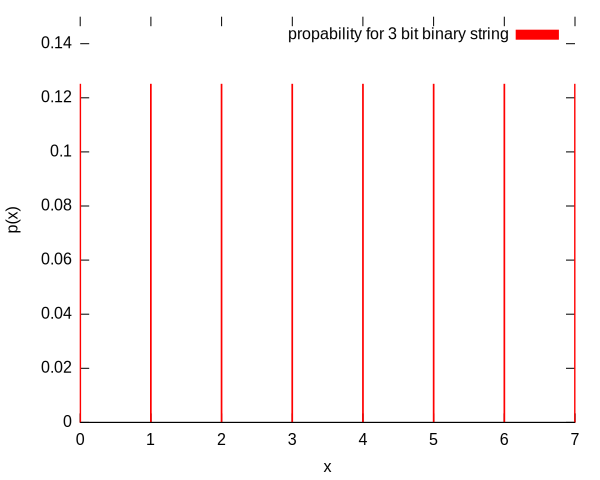
\includegraphics[width=0.6\textwidth]{figures/uniform}
    \caption{Uniform Distribution of binary string of length 3}
    \label{fig:uniform}
\end{figure}

\begin{figure}
    \centering
    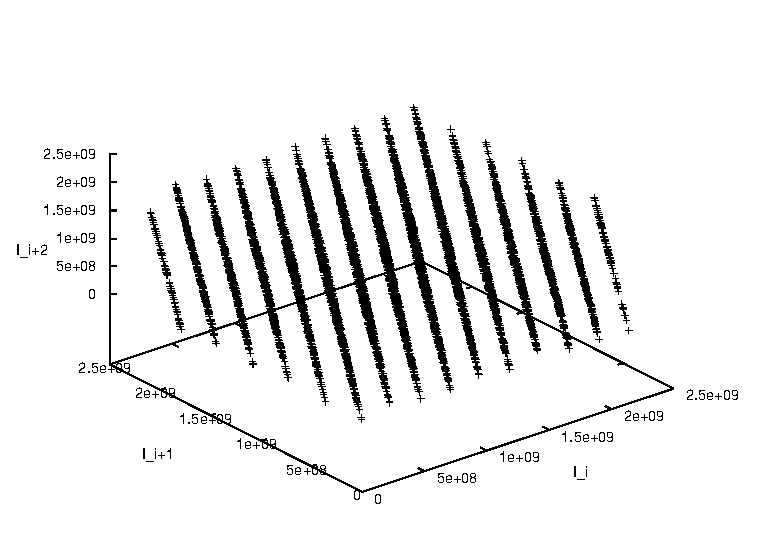
\includegraphics[width=1\textwidth]{figures/randu}
    \caption{Spectral Plot of RANDU output}
    \label{fig:randu}
\end{figure}


\section{Symmetric vs. Asymmetric Cryptography}

As stated above, two very fundamental differences regarding the key used in a cryptographic system can be found. Symmetric ciphers, where 
the same key is used for encryption and decryption, outperform its asymmetric counterparts in regards of data throughput by a factor of about 1000 \cite{5412055}.
Additionally, they need shorter keys to achieve the same level of security - both arguments encourage it's use in embedded devices because of its less computing
and memory demands.

The big disadvantage of symmetric ciphers is that the key must be known to sender
and receiver of the message \textit{before} secure communication can take place. This constitutes some kind of chicken-egg problem: to be able to send encrypted
data, the key must be distributed, i.e. a secure channel has to be setup first for key exchange. But if such a secure channel can be established, it could also be used
for transmitting the sensitive data themself.
\\

Asymmetric or public key cryptography solves the problem of key distribution by using two different keys, belonging to the same key pair: the \textit{private}
key must be be protected from disclosure, while the \textit{public} key can be published without harming security. For encryption, the public key of the receiver
is used, who in turn will use his private key to decrypt the message. 

To be able to take benefit from the advantages of booth schemes, a hybrid approach is possible: at first, public key cryptography is used to negotiate a symmetric session
key, which then can be used to encrypt the actual, sensitive data.

\subsection{Stream Ciphers}

Most stream ciphers belong to the family of symmetric ciphers, thus $e_i = d_i$. The reason is that most asymmetric ciphers are deterministic ciphers,
i.e. the encryption of the same message with a fixed public key always yields the same cipher text. Thus, such repeated messages can be detected by 
an adversary. 
Probabilistic public-key encryption can solves this problem for stream ciphers,
but this scheme will not be handled in this work because of its low practical application.

For encryption, stream ciphers take arbitrary long messages (from the message space $\mathcal{M}$), and encrypt
them to the corresponding ciphertext(out of the ciphertext-space $\mathcal{C}$), by applying
one digit of the message to one digit of the key. It is valid to say that a streamcipher is a block cipher with blocklength 1.

\begin{itemize}
 \item A keystream is a sequence of symbols $e_0, e_1, ..., e_n$, all taken from the keyspace $\mathcal{K}$
\end{itemize}

The encryption function $E_e$ performs the substitution $c_i = E_e(e_i, m_i)$, producing one encrypted symbol at a time. Analogously,
the decryption function inverts this substitution: $m_i = D_d(d_i, c_i)$.

\subsubsection{The Vernam Cipher} 

This cipher, also called \gls{otp}, was invented by Gilbert Vernam in 1918, and belongs to the family of polyalphabetic stream ciphers,
which means that every character of the origin message is mapped to another character of the same alphabet. In contrast to a monoalphabetical cipher,
there is no fixed mapping between the input and output characters.
The substitution is achieved by generating a keystream and by executing 
a bit-wise \gls{xor} operation, as defined in table \ref{table:xor}, of key and message.

\begin{center}
\begin{tabular}{ c c | c }
 \label{table:xor}
   &  & $\bigoplus$ \\ \hline
  0 & 0 & 0 \\
  0 & 1 & 1 \\
  1 & 0 & 1 \\
  1 & 1 & 0 \\
\end{tabular}
\end{center}

Decryption can be achieved by applying the \gls{xor} operation to key and ciphertext:

\begin{center}
 $m_i = c_i \bigoplus k_i = (m_i \bigoplus k_i) \bigoplus k_i = m_i$, with $ k_i \bigoplus k_i = 0, const \bigoplus 0 = const$
\end{center}


Obviously, the security of the cipher heavily depends on the quality of the \gls{prng}. If a truly random source is used to generate the key stream, this cipher
has perfect secrecy: for a n-character ciphertext, \textbf{all} n-character cleartexts are equally probable, and vice versa. 
The reason for this is the \gls{xor} operation: booth possible outcomes are booth equally probable, introducing one bit of randomness into every data bit. 

Additionally, the \gls{xor} operation can be built easily in hardware, accelerating the encryption or decryption process.

Nevertheless, the cipher can be completely broken if the same key is used for encrypting more than one cleartext message, allowing to mount
an attack based on frequency analysis.
If an attacker is able to intercept a high number of different ciphertexts, all encrypted with the same key, the pairwise xor'ing of the ciphertexts
yields the xor-combination of the corresponding cleartexts, because
\begin{center}
 $m_1 \bigoplus m_2 = (c_1 \bigoplus k) \bigoplus (c_2 \bigoplus k) = c_1 \bigoplus c_2 \bigoplus k \bigoplus k = c_1 \bigoplus c_2 \bigoplus 0 = c_1 \bigoplus c_2$
\end{center}

Whenever the same character is present in two different ciphertexts at the same position, the result of the \gls{xor} operation will be 0x00, allowing to draw
inferences about the language used. By utilizing frequency analysis, the used key can be determined position by position with effort bounded by $O(n^2)$.

\subsubsection{Stream Ciphers based on \gls{lfsr}}

An disadvantage of the Vernam cipher is that a key of equal length as the message is necessary. To mitigate this problem, a \gls{lfsr} can be used to generate
a key of proper length from a much shorter, initial key. Such \gls{lfsr} are denoted by $\langle L, C(D) \rangle$. $L$ is the number of stages, and $C(D)$ is the
\textit{connection polynomial}. Because of the finite length, every \gls{lfsr} can only take on a finite number of internal states, producing
a periodic output sequence.
If the degree of the connection polynomial is equal to the number of stages and the connection polynomial is irreducible (i.e. the polynomial can not
be factored into 2 non-constant polynomials), no matter of the initial state, the output sequence produced will always be of maximum periodicity.

Figure \ref{fig:lsfr} shows a 4 stage non-singular \gls{lfsr} with

\begin{center}
 $L=4$,  $C(D) = 1 + D + D^4$,
\end{center}

Table \ref{table:lfsr} \cite{handbookLFSR} shows the corresponding output sequence produced. After
15 shifts a state equal to the initial state is achieved, and the outputs
begin to repeat.

While such \gls{lfsr} can be easily built in hardware, a problematic fact remains that their \textit{linear complexity} is bounded by $L$. Therefore, a \gls{lfsr}
should never be used as keystream generator directly, instead the outputs of different \gls{lfsr} are combined by a non-linear function, thus obtaining a
nonlinear generator.

\begin{figure}
    \centering
    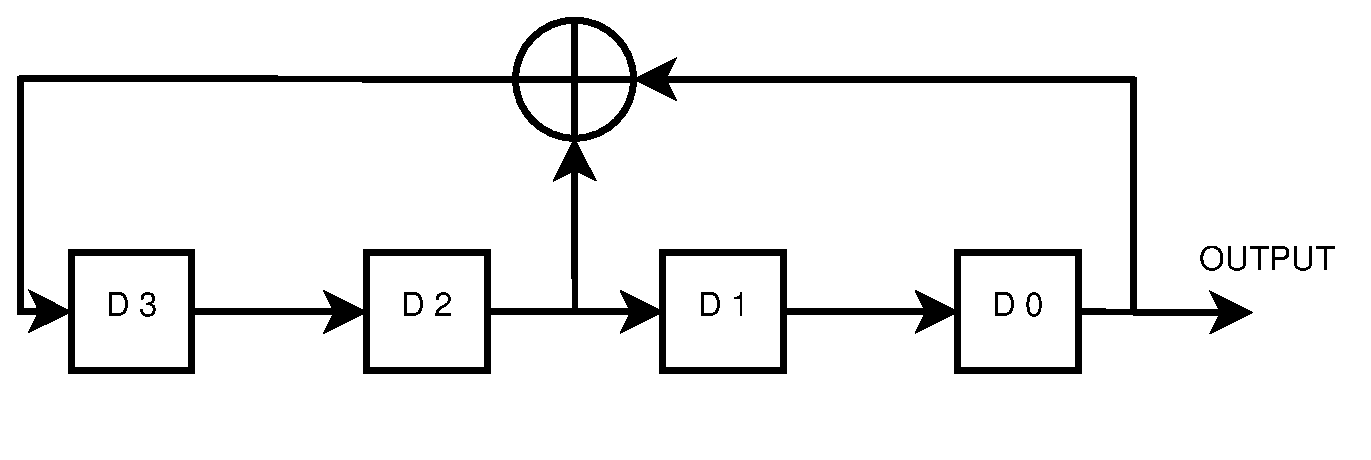
\includegraphics[width=1\textwidth]{figures/LSFR}
    \caption{4 Stage LFSR}
    \label{fig:lsfr}
\end{figure}

\begin{center}
\begin{minipage}{0.45\textwidth}
\begin{tabular}{ c | c | c | c | c }
 \label{table:lfsr}
  t & $D_3$ & $D_2$ & $D_1$ & $D_0$ \\ \hline
  0 & 0 & 1 & 1 & 0 \\
  1 & 0& 0& 1& 1\\
  2 & 1&0 &0 &1 \\
  3 & 0& 1& 0& 0\\
  4 & 0&0 &1 &0 \\
  5 & 0&0 &0 &1 \\
  6 & 1&0 &0 &0 \\
  7 & 1&1 &0 &0 \\
  \end{tabular}
\end{minipage}\hfill
\begin{minipage}{0.45\textwidth} 
\begin{tabular}{ c | c | c | c | c }
  t & $D_3$ & $D_2$ & $D_1$ & $D_0$ \\ \hline
  8  & 1& 1& 1& 0\\
  9  & 1& 1& 1& 1\\
  10 & 0& 1& 1& 1\\
  11 & 1& 0& 1& 1\\
  12 & 0& 1& 0& 1\\
  13 & 1& 0& 1& 0\\
  14 & 1& 1& 0& 1\\
  15 & 0& 1& 1& 0\\
\end{tabular}
\end{minipage}
\end{center}

\subsection{Block Ciphers}

These ciphers operate on input blocks of fixed size, transforming them into output blocks of same size. This implies that larger messages must be broken into
suitable blocks, and that for the last remaining block it may be necessary to add padding bytes to yield the full block size,
adding overhead to the message - a disadvantage compared to stream ciphers. For example, to encrypt a message just exceeding the block size by one byte,
for the excess byte a complete block must be concatenated. 

On the other hand, while stream ciphers are strictly sequential by nature, there exist methods to speed up block ciphers by splitting the message
first, and then process them in parallel\footnote{Counter Mode, see \ref{confidentiality}}. 
\\
Two main types of block cipher exist: \textit{transposition} ciphers use a key-dependent permutation to re-order the characters of the block to obtain the ciphertext.
This is a bijective transformation, so decryption can be achieved by simply reversing the permutation.

Substitution ciphers define a key-dependent mapping of characters from the alphabet $\mathcal{A}$ to the same alphabet, thus replacing every character by one
or more other characters. In the latter case, this equals an injective function which can not be reversed directly.
 
A product cipher is a combination of ciphers of different types to achieve a higher level of security than possible as with the basic ciphers. 
\\

Feistel networks are special product ciphers, composed of \gls{sp} networks. They were first described by Horst Feistel in the year 1973\cite{feistel}, and are 
the basis of a variety of block ciphers like "LUCIFER" \cite{feistel1974block,}, developed by Feistel, and \gls{des}.

Figure \ref{fig:feistel} shows the principal layout of such ciphers: at first, the plaintext block of length
2n-bits is divided into two n-bits blocks, often called $L_0$ and $R_0$ for left and right block, respectively. After that the first round starts: every round
is characterized by performing a substitution, followed by a permutation of the two half-blocks. For substitution, at first a \textit{round function},
parametrized by a \textit{round key} is applied to one half of the data block, followed by a \gls{xor} operation. The output of the rounds can be calculated
according to the formulas shown in \ref{table:feistel}
\\

\begin{center}
\begin{tabular}{ l l}
 \label{table:feistel}
  Encryption of round 1: & $L_1 = R_0$  \\ 
   &  $R_1 = L_0 \bigoplus F(k_1, R_0)$\\ \hline
  Encryption of round 2: & $L_{2} = R_1$  \\
   &  $R_{2} = L_1 \bigoplus F(k_2, R_1)$ \\ \hline
   ... &  \\ \hline
   Encryption of round n: & $L_{n} = R_{n-1}$ \\
   & $R_n = L_{n-1} \bigoplus F(k_n, R_{n-1})$ \\
\end{tabular}
\end{center}

Decryption is achieved by applying the ciphertext to the same network, with the round keys applied in reverse order, reducing hardware- respectively
code size, as shown in \ref{table:feistelRev}. Because decryption does not rely on reversing the round function, there is no necessity for the round function to be bijective.
\\

\begin{center}
\begin{tabular}{ l l}
 \label{table:feistelRev}
Decryption of round n: & $R_{n-1} = L_n$  \\
 & $L_{n-1} = R_n \bigoplus F(k_n, R_{n_1}) = R_n \bigoplus F(k_n, L_{n}) $
\end{tabular}
\end{center}

\begin{figure}
    \centering
    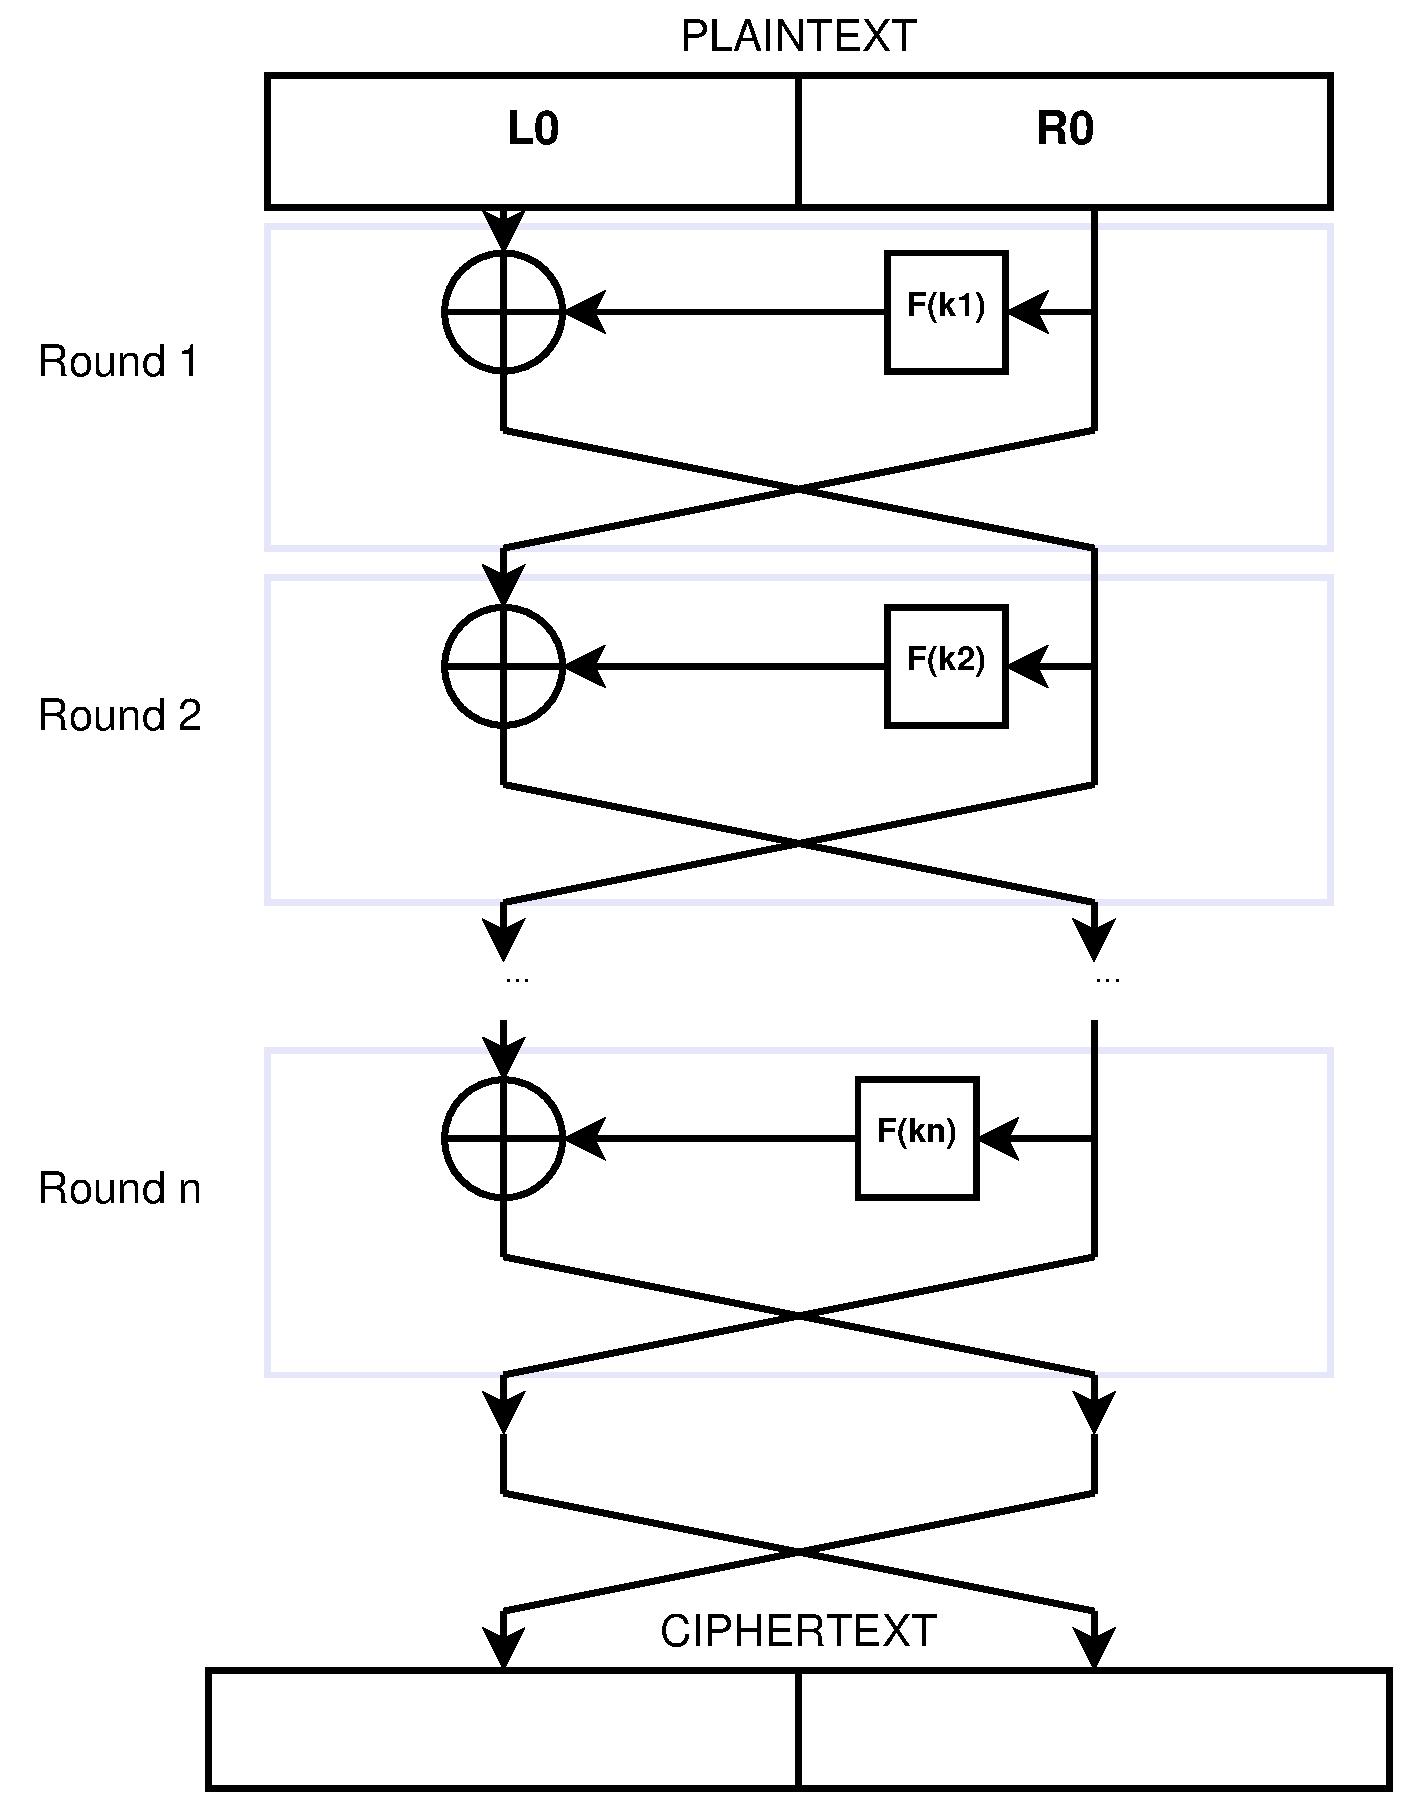
\includegraphics[width=0.5\textwidth]{figures/feistel.eps}
    \caption{Feistel Substitution-Permutation Network}
    \label{fig:feistel}
\end{figure}

\subsubsection{\gls{des} and \gls{3des}}

\gls{des}, designed by IBM and published by \gls{nist} in 1977 \cite{des}, encrypts 64 bit blocks in 16 processing rounds.

For every round, a 56 bit round key is derived from the basic 56 bit
key by permutations. The 64 bit data block to be encrypted respectively decrypted is subjected to an initial permutation and then feed into the Feistel
network. The round function operates as follows:

At first, the 32 bit half block is expanded to 48 bit by copying specific bits. The outcome is added to the round key modulo 2 (i.e., the \gls{xor} operation).
Next, a non-linear transformation is applied by so-called "S-Boxes", performing a surjective function by substituting blocks of 6 bit by only
4 bit. Lastly, a deterministic permutation follows, achieved through "P-Boxes", concluding the round
function.

Because of the small key size, \gls{des} was successfully broken for the first time\footnote{At least officially - rumors about the involvement of the \gls{nsa}
regarding the small key size and the design of the S-Boxes existed since the publication} by a brute-force attack in 1997.

To prevent such attacks, \gls{3des} was published: the cleartext- respectively 
cipertext block is feed 3 times to the \gls{des} cipher, using 3 different keys $k_1, k_2, k_3$ to first encrypt with $k_1$, decrypt with $k_2$ and finally 
encrypt with $k_3$, effectively tripling the key size:

\begin{center}
 $ciphertext = E(k_3(D(k_2,E(k_1, cleartext)))$
\end{center}

The special sequence of encryption, decryption and again encrypting was chosen because by setting $k_1 = k_2 = k_3$, a \gls{3des} implementation can also be used
for en/decryption of \gls{des} messages.

\subsubsection{\gls{aes}}

Also called "Rijndael" after its developers Joan Daemen und Vincent Rijmen, \gls{aes} is is the successor of \gls{3des}, as
proposed by the \gls{nist} in 2001. Basic properties are a block size of 128 bit, and possible key sizes
of 128, 192 or 256 bit.

The operation, shown in figure \ref{fig:aesEnc}, starts by copying the input block into a square matrix, called "State",
followed by a \gls{xor} combination of the first round 
key and the matrix. Then, 9, 11 or 13 rounds, depending on the key size, are performed: substitution by S-Boxes, permutation by shifting rows, 
another substitution by mixing columns and applying the round key. A last round, omitting the mix-columns stage, concludes the encryption.
Operating on the whole data block, \gls{aes} is not a Feistel network, therefore all substitutions and permutations must be reversible to allow decryption: 
the S-Box used here is therefore implementing byte-by-byte substitutions. The round keys are derived from the origin key by the \gls{aes} key expansion.

\begin{figure}
    \centering
    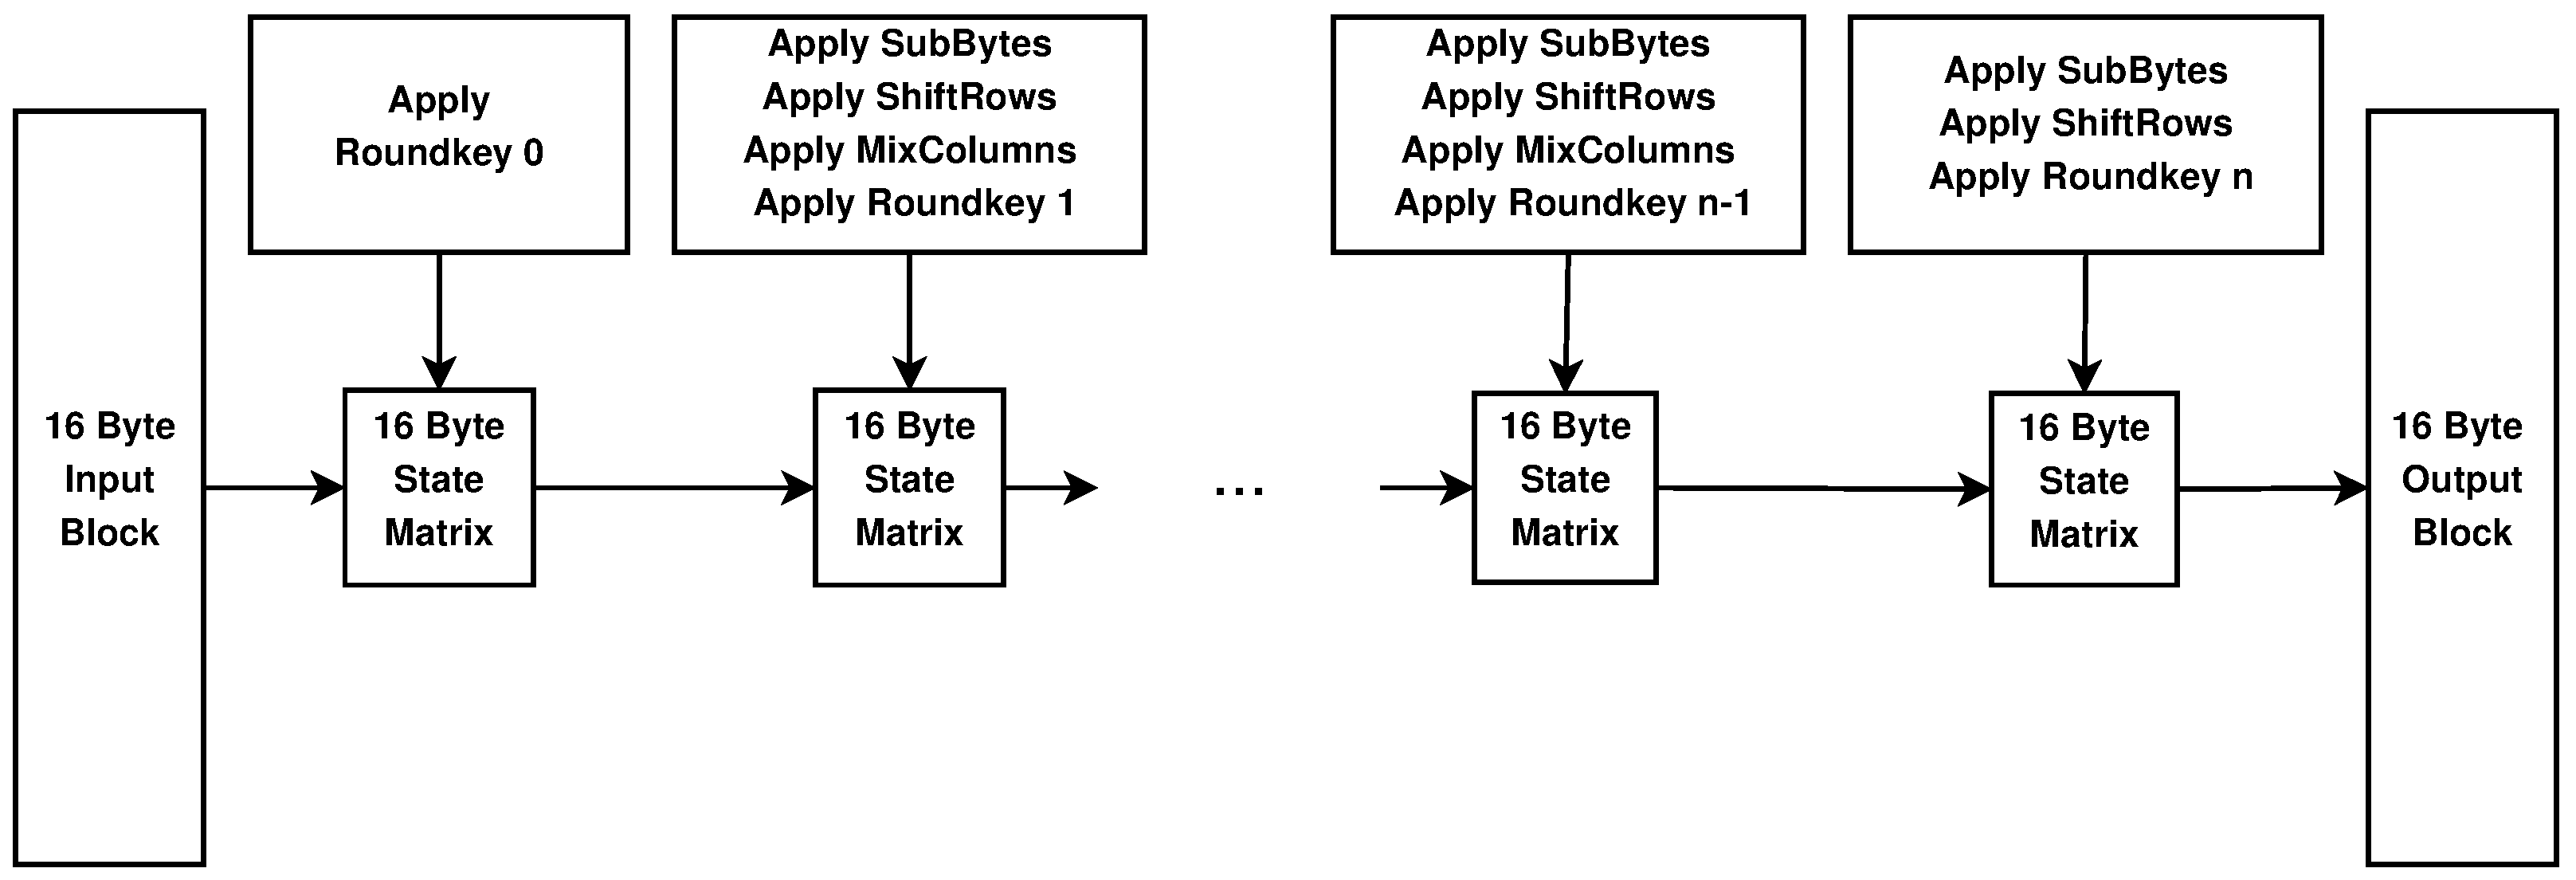
\includegraphics[width=1\textwidth]{figures/aesEnc.eps}
    \caption{AES Encryption Process}
    \label{fig:aesEnc}
\end{figure}

Decryption uses the round keys in reverse order. To reverse the first substitution of every round, a unique inverse S-Box is used, while the shifting rows
and mixing columns can also be reversed.
\\

FIXME: S-Box berechnung erklaeren?? stallings, principles and practice 

\subsection{Mode of Operation}\label{confidentiality}

Because block ciphers  operate on a fixed number of bytes, messages larger than this block size must be broken into parts of suitable size, and depending on 
the resulting size of the last block, it may be necessary to append a padding to it. Five different such modes were defined by \gls{nist} in 2001 \cite{moo},
which will be introduced in the next sections. For all modes it does not matter what underlying block cipher is used, as long as the block cipher implements
a cryptographic secure function. 

An important property of this modes is the error propagation.
Whenever a bit error occurs on the transmission channel due to noise or interference,
a logical '0' of the transmitted cipher text is substituted by a logical '1' or vice versa. This bit error in the cipher text produces one or more bit errors
in the clear text, thus the name error propagation \cite{burda}.

\subsubsection{\gls{ecb}}

\gls{ecb} can be used to gain confidentiality and allows the parallel processing of all input blocks. This mode does not use any \gls{iv} or nonce, therefore
repeating input blocks are mapped to the same output blocks under the same key. This is problematic, which can be seen quite intuitively by comparing 
figures \ref{fig:tuxclr} and \ref{fig:tuxecb}. Therefor this mode should be avoided.

 \begin{minipage}{\linewidth}
      \centering
      \begin{minipage}{0.4\linewidth}
          \begin{figure}[H]
              \includegraphics[width=\linewidth]{figures/TuxCleartext.png}
              \caption{Unencrypted Picture}
              \label{fig:tuxclr}
          \end{figure}
      \end{minipage}
      \hspace{0.05\linewidth}
      \begin{minipage}{0.4\linewidth}
          \begin{figure}[H]
              \includegraphics[width=\linewidth]{figures/TuxECB.png}
              \caption{\gls{ecb} encryption of the picture}
              \label{fig:tuxecb}
          \end{figure}
      \end{minipage}
  \end{minipage}

\subsubsection{\gls{cbc}}

This mode uses an \gls{iv} and can therefor be used for encryption of same messages without changing the key. Additionally, \gls{cbc} can also be used
for \gls{mac2} generation, as shown in section \ref{Integrity}.

Encrypting a message is shown in figure \ref{fig:cbc_encrypt}.

\begin{center}
$ C_0 = E(k, (M_0 \bigoplus IV ) )  $
\\
$ C_1 = E(k, (M_1  \bigoplus C_0) ) $
\\
$...$
\\
$ C_i = E(k, (M_i \bigoplus C_{i-1} ) )  $
\end{center}

To reverse the process, i.e. decrypt the message, see figure \ref{fig:cbc_encrypt}

\begin{center}
$ M_0 = D(k, C_0) \bigoplus IV $
\\
$ M_1 = D(k, C_1) \bigoplus C_0 $
\\
$...$
\\
$ M_i = D(k, C_i) \bigoplus C_{i-1} $
\end{center}

The \gls{iv} does not have to be kept private, but must be known to the receiver of the message. It is important that such an \gls{iv} is unpredictable, otherwise
allowing a \gls{cpa}. Also, it must not repeat over the lifetime of the key, otherwise introducing the \gls{ecb} problem again. 

The \gls{iv} introduces overhead, which is more problematic for  shorter messages.
To avoid such a message expansion, a solution is to use a "nonce", which stands for "\textit{n}umber used \textit{once}", as suggested in \cite{cryptoEng}.
Sender and receiver must maintain a message counter. This message counter must be encrypted to avoid predictability, and can then be used as \gls{iv}. Care must
be taken for the counter not to overflow within the lifetime of a key.

\begin{figure}
    \centering
    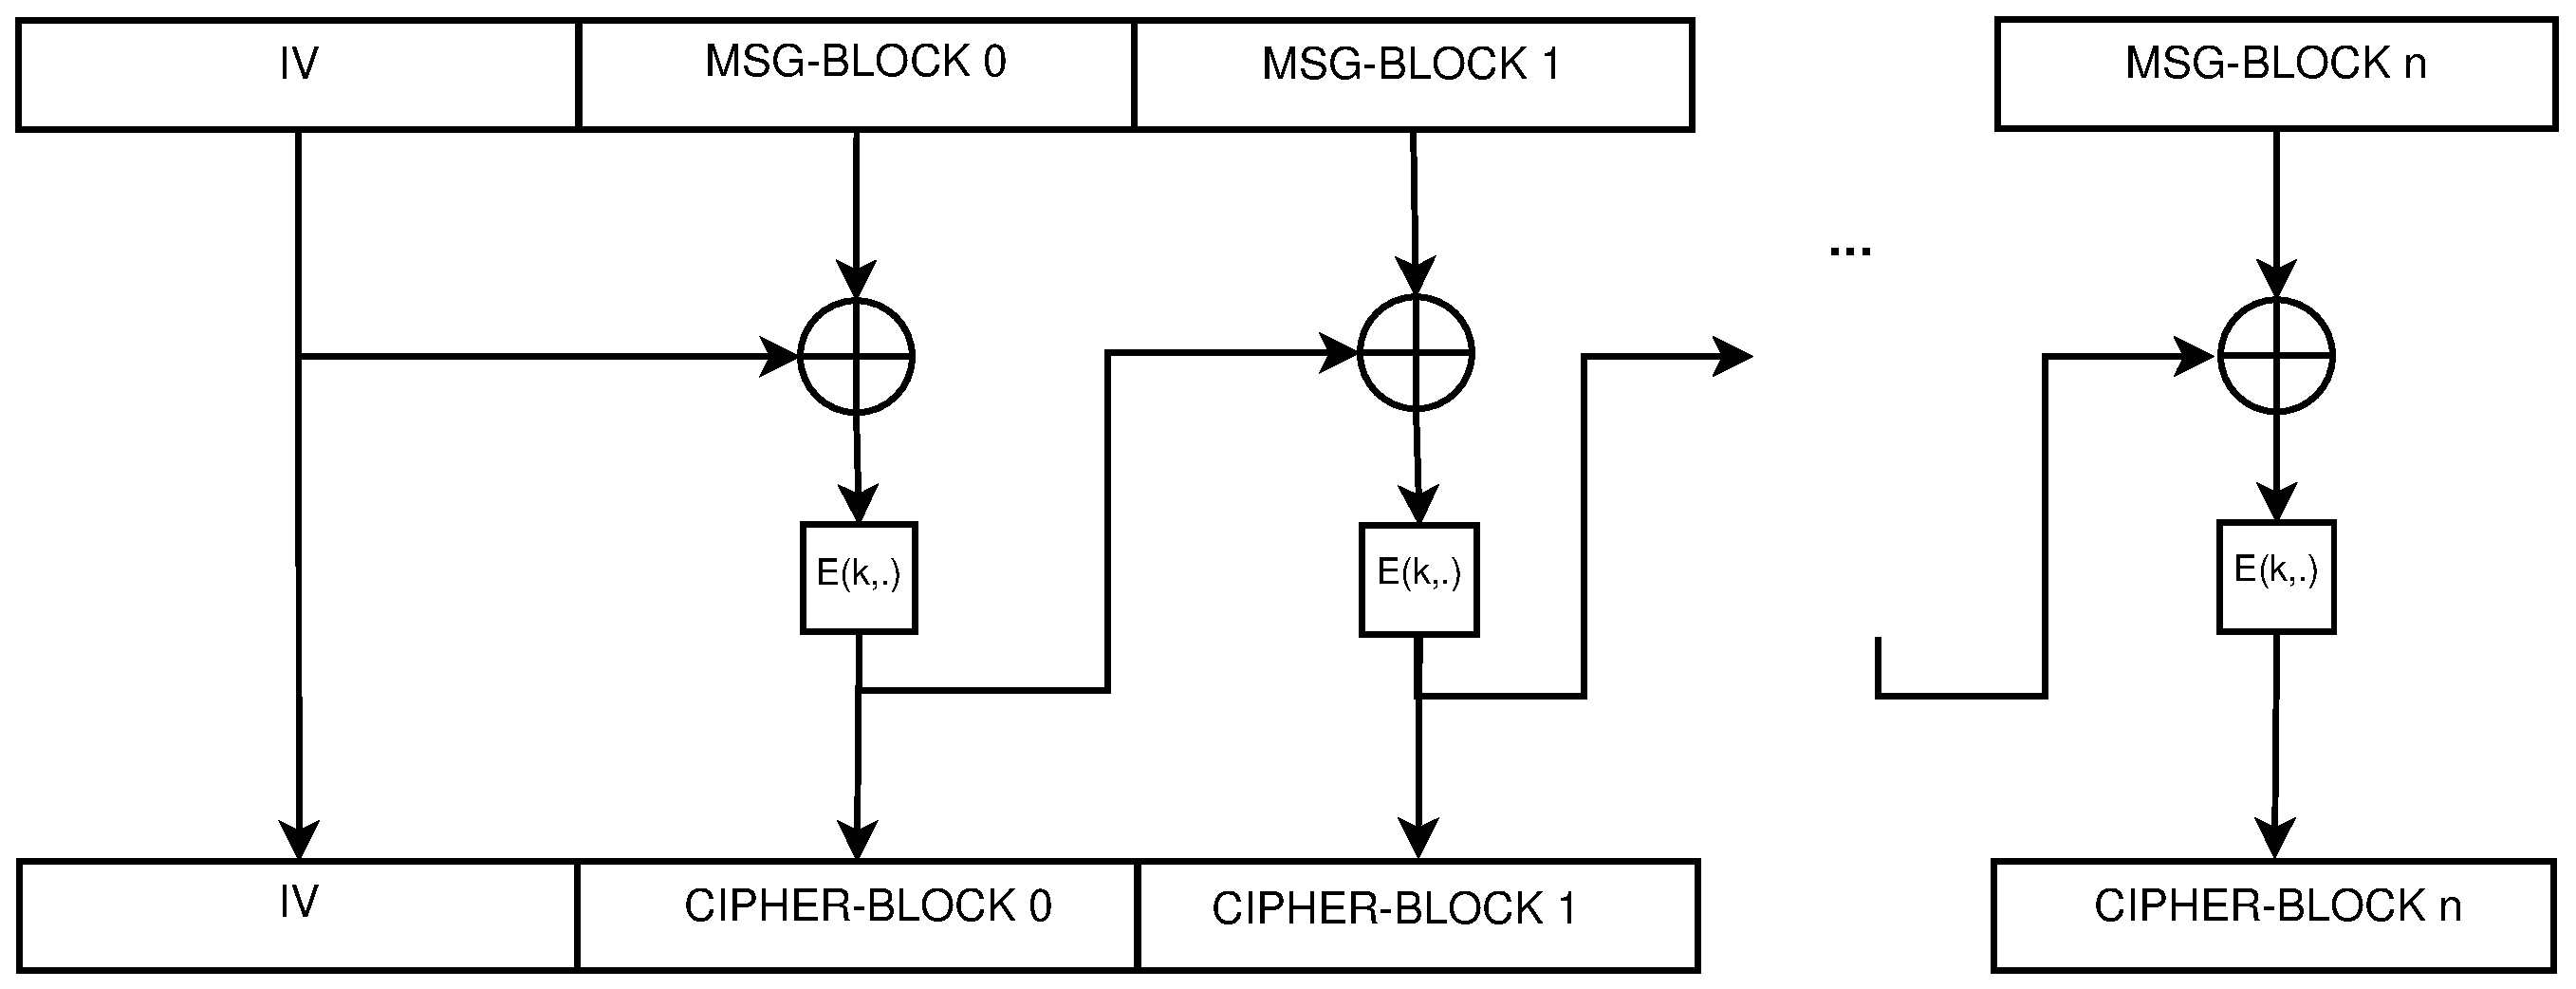
\includegraphics[width=1\textwidth]{figures/CBCencrypt.eps}
    \caption{Cipher Block Chaining for encrypting messages}
    \label{fig:cbc_encrypt}
\end{figure}

\begin{figure}
    \centering
    \includegraphics[width=1\textwidth]{figures/CBCdecrypt.eps}
    \caption{Cipher Block Chaining for decrypting messages}
    \label{fig:cbc_decrypt}
\end{figure}

\subsubsection{\gls{ctr}}

This confidentiality mode generates a key stream by encrypting a counter value with a block cipher. The key stream is then applied to the cleartext
blocks with the \gls{xor} operation, as shown in figure \ref{fig:ctr}. For the last block, the key stream is truncated to match the size of the cleartext block.

Decryption works by generating the same key stream on the receiver's side, and applying the \gls{xor} operation to the ciphertext blocks, similar to the
decryption process used in the Vernam cipher.

\begin{figure}
    \centering
    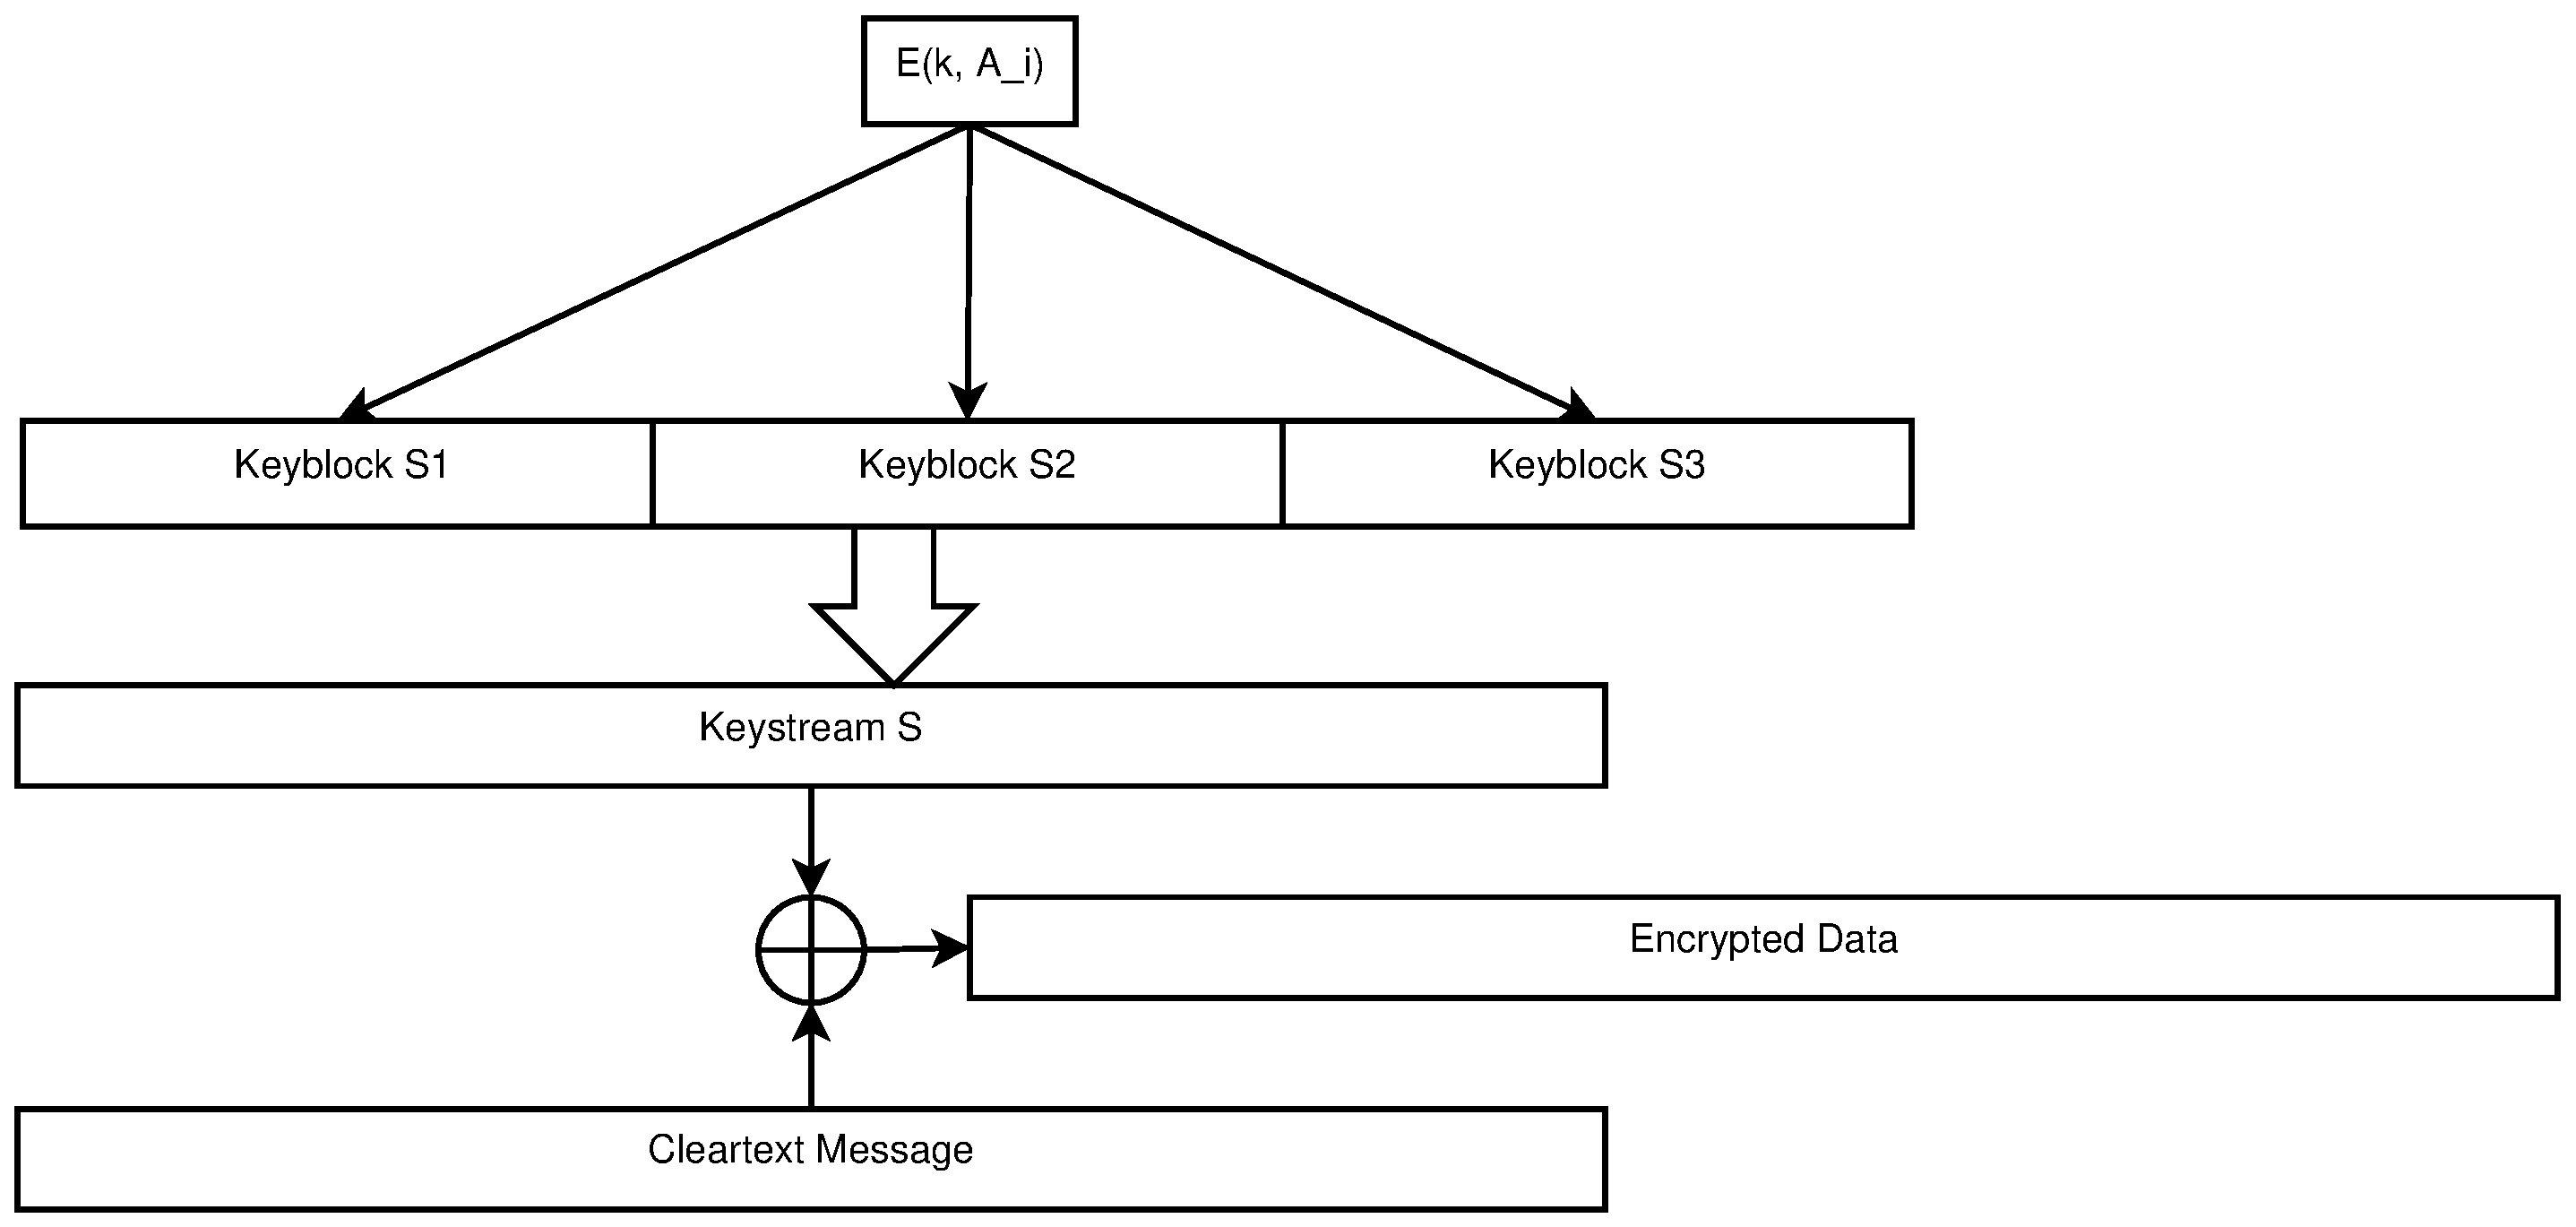
\includegraphics[width=1\textwidth]{figures/CTR.eps}
    \caption{CTR Encryption}
    \label{fig:ctr}
\end{figure}

To avoid the duplicate usage of the same counter value in bidirectional communication, the counter can be combined with a sender-dependent nonce by
concatenation before encrypting the counter:

\begin{center}
 $K_{0} = E(k, nonce || Ctr_0)$\\
 $K_{1} = E(k, nonce || Ctr_1)$\\
 ...\\
 $K_{i} = E(k, nonce || Ctr_i)$\\
 $C_i = K_i \bigoplus M_i$
\end{center}
 
\subsubsection{\gls{cfb}}

\gls{cfb} can be used to turn a block cipher into a stream cipher. Beside the block size $b$, another parameter $s$ determines the operation. $s$ corresponds
to the size of one transmission unit. For initialization, an unpredictable \gls{iv} is set as input for the underlying block cipher. Then, in every
processing step a new transmission unit is generated by \gls{xor}ing the $s$ most significant bits
of the output of the encryption function with the $s$ bit message unit. After that, the \gls{iv} is shifted to the left and the gap is filled
by the newly generated character, as shown in figure \ref{fig:cfb}:
\\
\\
 $C[0] = E(k, IV[0:b-1])[b-1:b-s-1] \bigoplus M[0]$\\
 $C[1] = E(k, IV[0:b-s-1] || C[0])[b-1:b-s-1] \bigoplus M[1]$\\
 ... \\
 $C[n] = E(k, IV[0:b-ns-1] || C[0] || C[1] || .. || C[n-1])[b-1:b-s-1] \bigoplus M[n-1]$\\
\\

To decrypt, the same encryption function, \gls{iv} and key is used to retrieve one transmission unit at a time.
 
\begin{figure}
    \centering
    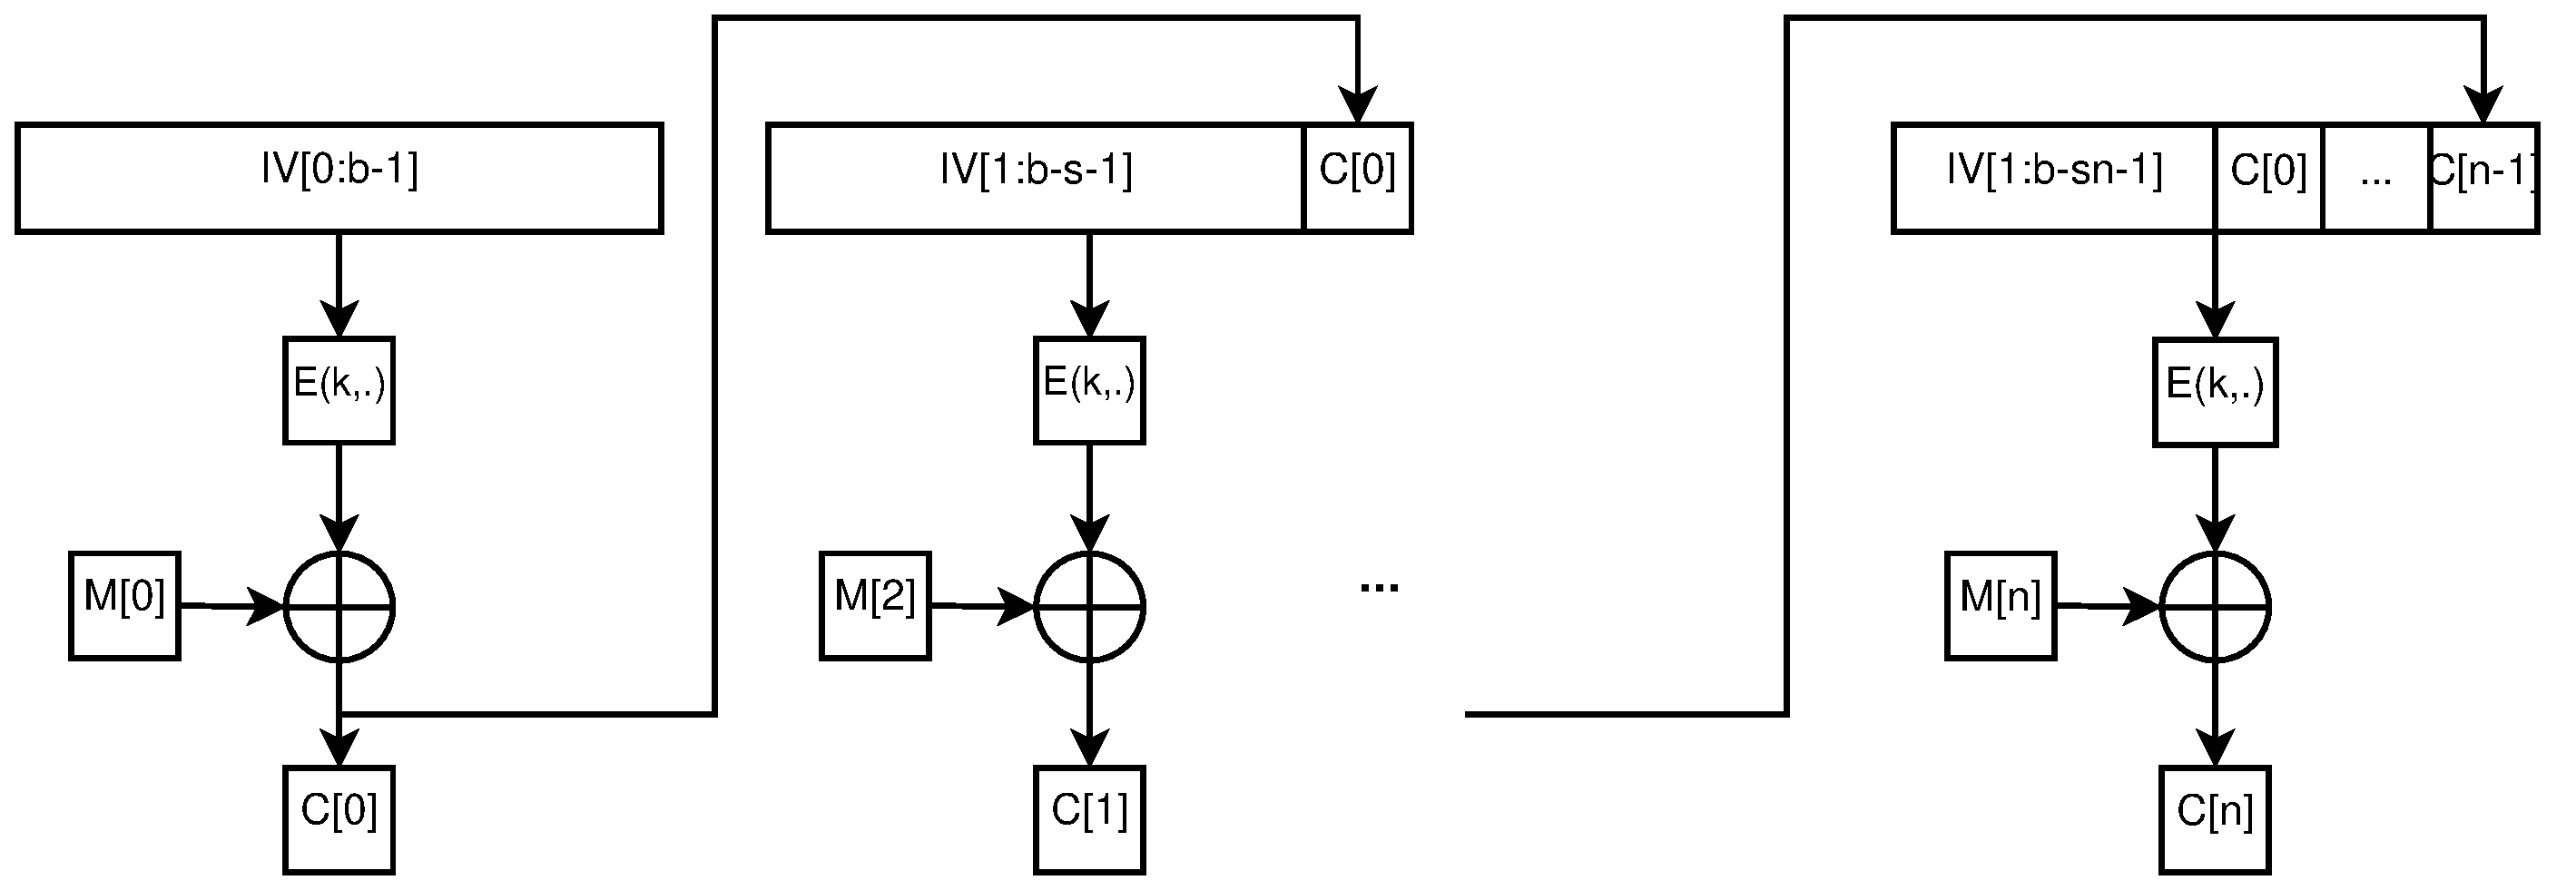
\includegraphics[width=1\textwidth]{figures/CFB.eps}
    \caption{CFB Encryption}
    \label{fig:cfb}
\end{figure}

\subsubsection{\gls{ofb}}

This mode is very similar to \gls{cfb}, but here the $s$ bit output from the encryption function is used directly to update the space caused by the \gls{iv} 
left shift. This avoids error propagation in case a transmission unit was damaged on transmit and thus a bit changed its value:
for \gls{ofb} encryption systems, one or more bit errors in one ciphertext character only affects the decryption of this character. In contrast, one bit error in \gls{cfb} affects
decryption of all following characters.
\\
\\
$O_0 = E(k, IV[0:b-1])[0:s-1]$\\
$C[0] = O_0 \bigoplus M[0]$\\
 $O_1 = E(k, IV[0:b-1] || O_0)[0:s-1]$\\
 $C[1] = O_1 \bigoplus M[1]$\\
 ... \\
 \\
 $0_n = E(k, IV[0:ns-1] || O_0 || O_1 || O_{n-1})[0:s-1]$\\
 $C[n] = O_n \bigoplus M[n]$\\

\begin{figure}
    \centering
    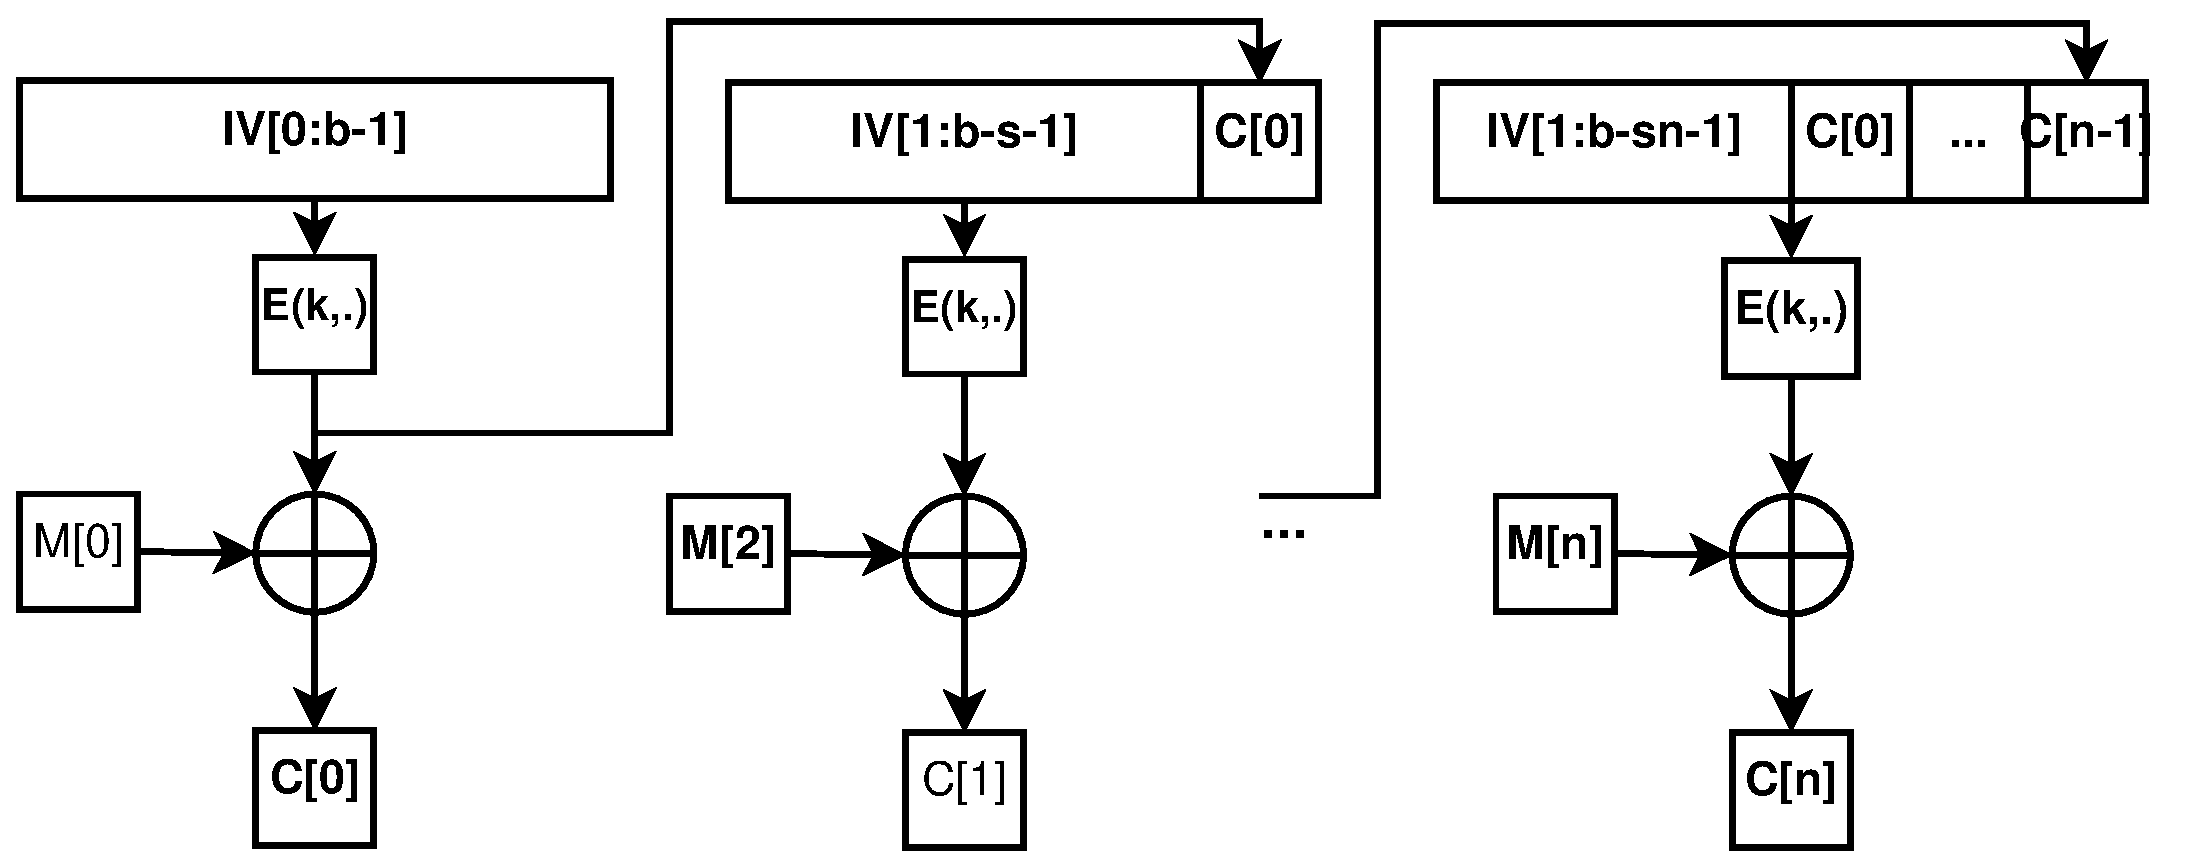
\includegraphics[width=1\textwidth]{figures/OFB.eps}
    \caption{OFB Encryption}
    \label{fig:ofb}
\end{figure}

\subsubsection{Integrity}\label{Integrity}

All modes of operation introduced so far are used to provide confidentiality only. To provide the second column of information security, i.e. integrity, in general
\glspl{mac2} or digital signatures are used.
Digital signatures are based on public key cryptography and are introduced in section \ref{digitalSignatures}. In contrast, \glspl{mac2} use symmetric keys,
providing integrity and authenticity. 
\\
The basic way to protect a data unit - be it a message traveling from sender to recipient or a file saved for later usage - from modification by a third party is to
generate a tag $t$, also called \gls{mac2}, and concatenating this tag to the message, as shown in figure \ref{fig:tag}.
Verifying the integrity is done by re-generating the tag and comparing it to the saved on. 
\\
\\
Integrity means that a data unit is 
protected from tampering by third parties in a way that such a modification by an unauthorized entity is detectable. Authenticity means that the receiver of
a message can verify that the message really was sent from the sender and not by an illegitimate third entity. Obviously, this two concepts are semantically
related: checking the integrity implicitly checks authenticity, provided that the key used to generate the tag is only known to authentic entities.
\\
Vice versa, authenticating the sender of a message is only useful if the message itself cannot be modified by an adversary, i.e. integrity is guaranteed. To
avoid confusion, the term integrity is used if the meaning is clear from the context.
\\
\\
In contrast to confidentiality modes, which should always be combined with a method to guarantee integrity (as shown in FIXME), 
integrity-only modes do have a right to exist. For example, archives containing source code for open source project, available from the internet, must not be
encrypted but should be secured against modification. For example, the UNIX based operating system "FreeBSD" uses asymmetric keys to protect it's package
management system from adversary modification.
\\
\\
Combining integrity and confidentiality in a security scheme called \gls{ae} will be handled in section \ref{authEncrypt}.
\\
\\
As tag generation and tag verification algorithms, keyed or unkeyed cryptographic secure hash functions are used.
For integrity-only, keyed hash functions must be used, or
otherwise an arbitrary entity can modify the message undetectable by regenerating the correct tag. Therefor, a simple checksum like a \gls{crc} or an unkeyed 
hash function can not provide integrity only, simply because the function value can be re-generated by an adversary modifying the message, allowing to mount
an attack called \gls{mac2} forgery.
Nevertheless, in combination with a confidentiality mode such an unkeyed function \textit{may} be secure, although it's use is discouraged because many applications operating
this way are broken and can be attacked (i.e. \gls{ssh} version 1 \cite{zalewskissh}).
\\
\\
A hash functions takes as input an arbitrary large message $\mathcal{M}$ and generates a hash value $t = h(\mathcal{M})$ of fixed size, therefor $|M| >> |t|$. This many-to-one
mapping implies the existence of collisions, i.e. the existence of distinct messages $m_1, m_2$ which are mapped to the same tag $t$.
\begin{figure}
    \centering
    \includegraphics[width=0.5\textwidth]{figures/tag.eps}
    \caption{Tag generation}
    \label{fig:tag}
\end{figure}
\\
\\
To be cryptographically secure, a hash function must fulfill specific properties \cite{6732428}: firstly, while it should be easy to generate the tag
by calculating $t = h(m)$, reversing the process to get $m$ by executing $h(t)^{-1}$ should be hard, a property called \textit{preimage resistance}. 
Additionally, \textit{2nd-preimage resistance} assures that for any given message $m$ and corresponding tag $t$, it must be infeasible to find a second message
that maps to the same tag. Finally, \textit{(strong) collision resistance} states that it also must be infeasible to find any two messages generating
the same tag, therefore collision resistance implies 2nd-preimage resistance \cite{handbookCR}.
\\
\\
Important representatives of cryptographically secure hash functions are the family of \glspl{sha}, with variants providing hashes of 160, 256, 384 or 512 bit 
length, defined by \gls{nist} \cite{nistSHA}. For \gls{sha}-1, an attack to find collisions was found \cite{Wang05findingcollisions} and should therefor not
be used anymore.
\\
Because these hash functions lack a secret key and therefor would allow \gls{mac2} forgery, a construction called \gls{hmac} can be used, which takes 
additionally to the message $m$ as input a key $k$, and $ipad$ and $opad$ being constant values \cite{hmac}.

\begin{align}
 t = S(k, m) = h((k \bigoplus opad) || h((k \bigoplus ipad) || m)) 
\end{align}
\\
\\
A different way for tag-generation, called \gls{cbc}-\gls{mac2}, is based on block ciphers, utilizing a construction similar to \gls{cbc} mode encryption,
shown in figure \ref{fig:cbc_MAC}. 

\begin{figure}\label{cbcMAC}
    \centering
    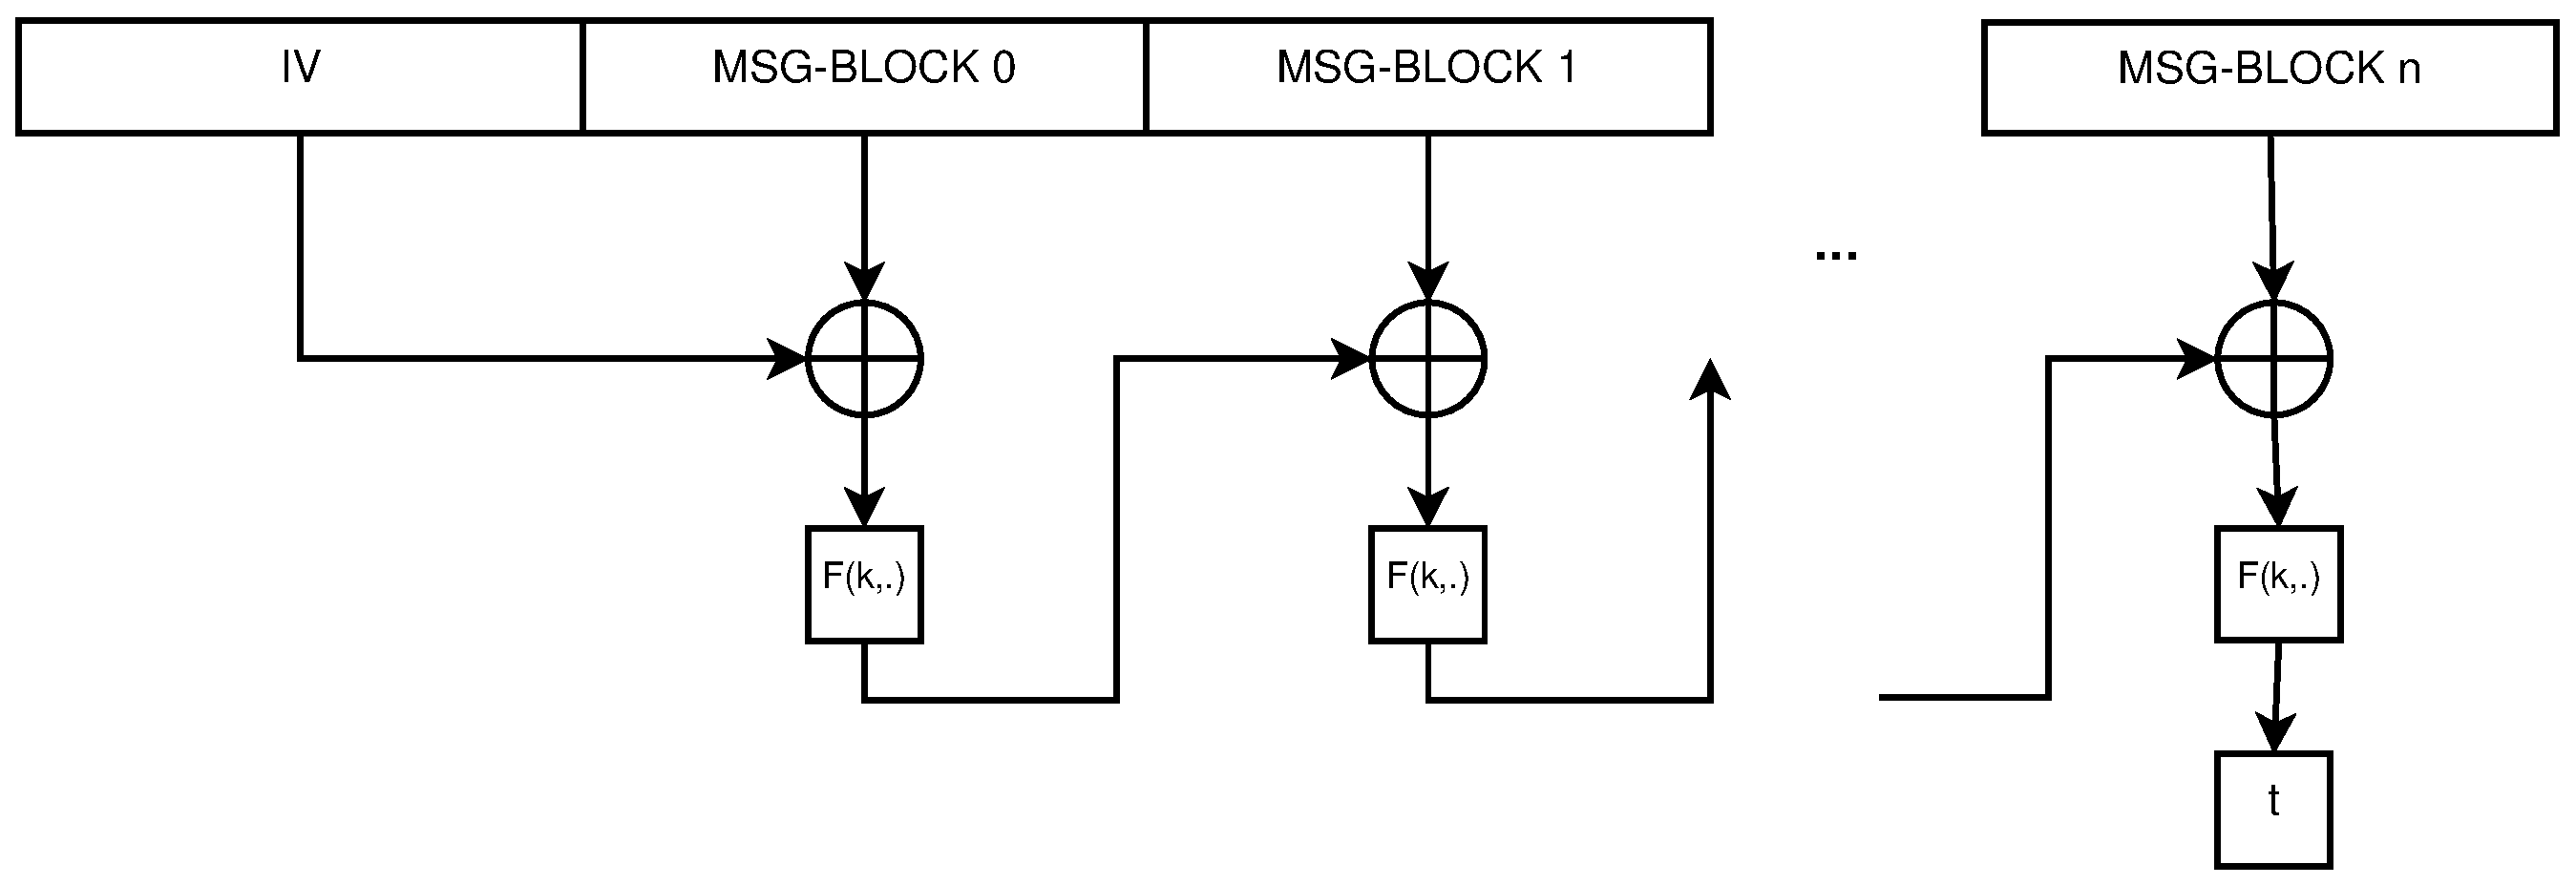
\includegraphics[width=1\textwidth]{figures/CBCMac.eps}
    \caption{Cipher Block Chaining for generating a MAC}
    \label{fig:cbc_MAC}
\end{figure}

\begin{figure}\label{cbcMACFlags}
    \centering
    \includegraphics[width=0.5\textwidth]{figures/CBCIVFlags.eps}
    \caption{Flag Field of CBC IV}
    \label{fig:cbc_Flags}
\end{figure}

\section{Authenticated Encryption}\label{authEncrypt}

Many applications demand the integration of confidentiality \textit{and} integrity modes. The need for confidentiality is self explaining in systems where
submitted data must be protected from a passive adversary. One example would be a password for logging into a remote computer, sent over a network connection
- just by monitoring the connection, an attacker can steal the password and gain illegitimate access to the system.
\\
\\
The need to additionally provide integrity and authenticity measurements is maybe not that obvious, but can be motivated in various ways. For example, two entities
sharing an initial key known to booth of them which want to negotiate a temporary session key could randomly choose the temporary key, encrypt it and send it
to the other side. Even if a passive adversary knows that the package he monitors will be used as session key he cannot derive it, provided a secure cipher is
used.  In contrast, an active attacker can intercept and modify the encrypted session key, and afterwards inject the modified message. The receiver
would then decrypt the package, thus obtaining a modified session key. After all, the two entities would use two different keeps, crippling their communication.
\\
More precise arguments can be found for different modes of operation, as introduced above. FIXME: ENCRYPTION ONLY ATTACKS
\\
\\
To avoid that attacks, methods to provide encryption and integrity are combined. Basically, 3 different ways how this can be achieved exist:

\begin{itemize}
 \item "encrypt-and-mac" encrypts the message $m$ and appends the tag $t$ of the cleartext message
 \begin{align}\label{encAndMac}
  c = E(k_e, m) || h(k_h, m)
 \end{align}
 \item "mac-then-encrypt" generates the tag for the cleartext message $m$, appends it and afterwards encrypts cleartext + tag to get ciphertext $c$:
 \begin{align}\label{macThenEnc}
  c = E(k_e, m || h(k_h, m))
 \end{align}
 \item "encrypt-then-mac" encrypts the message $m$ first, and afterwards appends the tag $t$ of the encrypted message to obtain $c$
 \begin{align}\label{encThenMac}
  c = E(k_e, m) || h(k_h, E(k_e, m))
 \end{align}
\end{itemize}

For all 3 schemes, $E(k, m)$ must be a semantically secure encryption function, and $h(k, m)$ denotes a keyed, cryptographically secure hash function.
The latter is of particular importance for \ref{encAndMac}, because this scheme otherwise directly leaks information about the plaintext in the tag. 
\\
It turns out that only \ref{encThenMac} is considered generically secure against chosen plaintext attacks.
In contrast, "encrypt-and-mac" \cite{sshBellare}, used in \gls{ssh}, is considered generically
insecure. For "mac-then-encrypt", used in \gls{ssl}, the same holds true, but this scheme can be used in a secure manner if \gls{cbc} or a stream cipher like 
\gls{ctr} mode is used for encryption. 

\subsection{CCM}

CCM\footnote{http://tools.ietf.org/html/rfc3610}, short for \textit{Counter with CBC-MAC} combines CBC for authentication and CTR mode for encryption.
CBC generates the MAC for the message first, appends this MAC to the cleartext data and afterwards encrypts data + MAC with counter mode, thus using a
\textit{MAC-then-Encrypt} scheme. The only
supported block size is 128-bit blocks, so it is possible, but not mandatory, to use 128-bit AES as underlying block cipher.
\\
Two application dependent parameters have to be fixed first: 
\begin{itemize}
 \item M: Number of octets in the MAC field. A shorter MAC obviously means less overhead, but it also makes it easier for an adversary to guess the correct
 value of a MAC, so valid values are $M \in \{4, 6, 8, 10, 12, 14, 16\}$. FIXME: shorter MACs insecure, border=4 ? 
 \item L: Number of octets in the length field. This is a trade-off between the maximum message size and the size of the nonce. Valid values are $2 \leq L \leq 18$.
 For example, when setting $L = 2$, 2 bytes are reserved for the length field, which means that the biggest message that can be encrypted is of size 64kB. The actual
 length of the message is filled into the field named 'length(msg)', as shown in figure \ref{fig:cbc_MAC}.
\end{itemize}

Both parameters are encoded in the very first byte of the first message block, thus reducing the possible maxium size of the nounce, as shown in figure \ref{fig:cbc_Flags}.
Bit 6 of the length field is set to 1 if additional authenicated data(FIXME) are sent, and bit 7 is reserved and set to 0.


\subsubsection{Generating the MAC}

As shown in chapter \ref{authenticity} in figure\ref{fig:cbc_MAC}, the first message block $M_0$ is \gls{xor}'d with a nonce or initialization vector(IV, see figure
\ref{fig:ccrMacIV}), which \textbf{must be unique per key}.FIXME
The result of the \gls{xor} operation is then feed to the block-cipher to get the first cipherblock $C_0$. The encrypted data $C_0$ gets \gls{xor}'d with the next message block $M_1$, and this
result becomes the input for the block cipher, and so on, iterating over all $n$ message blocks to determine the tag $t$:

\begin{figure}
    \centering
    \includegraphics[width=0.5\textwidth]{figures/"CCM CBC IV".png}
    \caption{IV for CBC MAC}
    \label{fig:ccrMacIV}
\end{figure}


\begin{center}
 $C_0 = F(k, M_0 \bigoplus IV )$
 \\
 $C_1 = F(k, M_1 \bigoplus C_1) $
 \\
 $...$
 \\
 $C_n = F(k, M_n \bigoplus C_{(n-1)})$
 \\
\end{center}

The resulting tag $t$ can be truncated, corresponding to the chosen MAC size $M$:
\begin{center}
  $t = C_n[M:0]$, with $M \in \{4, 6, 8, 10, 12, 14, 16\}$
\end{center}
which means that the tag $t$ consists of the least significant $M$ bytes of the output of the last encryption block.

\subsubsection{Encrypting Data and MAC}

Counter-mode is used for encrypting the actual payload and the concatenated, CBC mode generated MAC.
Thus, authenticated encryption is achieved in a manner also called 'mac-then-encrypt'. While authenticated
encryption modes implementing this ordering(generate mac first, then encrypt data and mac) \textit{may}
be vulnerable to padding oracle attacks(FIXME), counter mode effectively avoids these simply because
there is no padding needed, as will be shown.

Counter mode implements a weaker form of the one time pad by generating a keystream of sufficient
length, and then applying the \gls{xor} operation to the keystream and the data, as shown in figure \ref{fig:ctr}.


First, keyblocks with 16 byte length each are generated by encrypting the nounce, a flag and a counter with the key. These 
keyblocks are then concatenated and trimmed to the proper length (i.e., the length of the message to encrypt). This obtained keystream
is then bitwise \gls{xor}'ed with the cleartextmessage (which consists of the data and the MAC), yielding the final encryption.


\section{Public Key Cryptography}\label{pkc}

Public Key Cryptography solves the problem of establishing a secure channel by using an insecure one.
Here sender and recipient use two different keys: one for encryption, called \textit{public key}, the other
for decryption, called \textit{private key}. This key pair belongs together, hence this scheme is also called \textit{asymmetric} encryption. A fundamental requirement
is that it must be hard
to derive the decryption key from the encryption key. This behavior is achieved by some kind of public known one-way function where it is computationally
easy to calculate the result of $f(x) = y$, but only given $y$, it is computationally - in the domain of processing power and/or memory - hard
to reverse this function to get $x$.
The basic idea for such a one-way function was formulated for the first time in the year 1874 by William Stanley Jevons stating:
\\
\\
\textit{"Can the reader say what two numbers multiplied together will produce the number 8616460799? I think it unlikely that anyone but myself will
ever know."} \cite{wStanley} 
\\
\\
Although his statement was not related to cryptography at all, and of course factoring of much bigger numbers is doable nowadays, this statement exactly describes
the spirit of public key systems, and the security of RSA, introduced below, is directly connected to the inability to factor large numbers in reasonable time.

Because disclosure of the public key does not affect the security of the scheme, the public key can be published in some sort of dictionary.
An entity wanting to send an encrypted message to a receiver can then look up the receiver's public key, encrypt the message and send the resulting
ciphertext to the recipient, who then can decrypt the message. 
\\
\\
It is remarkable that any algorithm establishing public keys must authenticate it's participants, or it will be vulnerable to man-in-the-middle attacks.

\subsection{Merkle Puzzles}
In \cite{Merkle}, Ralph C. Merkle developed an algorithm for key exchange between two parties. While the algorithm is based on symmetric ciphers and is
not practicable, it motivates the usage of public key systems based on algebraic structures and is therefor introduced.
\\
\\
The key idea is that the necessary work by the two legitimate parties when negotiating a key is bounded by $O(n)$, while an adversary must spend $O(n^2)$ to 
also calculate the key, thus generating a quadratic gap. 
Merkle defines a puzzle as cipher text that is supposed to be broken. This can be achieved by restricting the size of the symmetric key used such that an
exhaustive search can be finished in feasible time. Every puzzle contains an id and a session key, booth chosen randomly, as well as a static string,
known to all participants.
\\
The party initiating the key exchange, called $X$, generates $n$ such puzzles and sends all of them to the receiver $Y$. $Y$ picks one puzzle at random and
decrypts it by trying all possible keys. Because of the static string inside the puzzle, $Y$ knows for sure when the correct key has been tried.
$Y$ then extracts the session key and sends the corresponding id back to $X$. Subsequently, booth parties can use the session key referenced by the id for encryption.
An eavesdropper $Z$, monitoring all puzzles, cannot directly determine which of them is containing the returned id and therefor does not know the session key the 
two parties agreed on - the only possibility for $Z$ is to attack \textbf{all} puzzles, squaring the effort spent by $X$ and $Y$.
\\
If, for example, one puzzle can be broken by $2^{32}$ computations, and $2^{32}$ different puzzles are used, $X$ must prepare, save and send $2^{32}$ puzzles
to $Y$, who in turn must try $2^{32}$ different keys. $Z$ must crack all $2^{32}$ puzzles, each with effort $2^{32}$, thus resulting in $2^{64}$ processing steps.
\\
While this algorithm is very wasteful in regards of processing power, memory and communication capacity, such a protocol would be useful if a more-than-quadratic
blowup could be achieved, but unfortunately, for all algorithms based on symmetric ciphers, this quadratic gap is the best that can be achieved,
as shown in \cite{Barak09merklepuzzles}.   
\\
 
To further increase the effort an attacker has to spend a different approach has to be found. It turns out that hard mathematical problems exist that are 
suitable for such a purpose. 
Therefor, in the next sections three important public key algorithms are introduced: \gls{dh} key exchange, based on prime fields, \gls{ecc}, and RSA.
The former 2 of them are based on finite fields, therefore a short mathematical introduction is given first.

\subsubsection{Finite Fields}\label{finiteFields}

A field consists of a set $\mathcal{F}$ together with two operations $\cdot$, namely addition "+" and multiplication "*", satisfying the following properties:

\begin{itemize}
 \item  Closure: for all elements from $\mathcal{F}$, the set is closed under the defined operations, i.e. applying an operator $\cdot$ to two elements from the set results in an
element also belonging to the set.
 \item Associativity and Commutativity hold, i.e. $a \cdot (b \cdot c) = (a \cdot b) \cdot c$ and $a \cdot b = b \cdot a$
 \item For both operations and all elements from the set $\mathcal{F}$ an identity element $e$ exists s.t. $a\cdot e = a$
 \item For both operations and all elements from the set $\mathcal{F} \backslash \{0\}$ an inverse element exists s.t. $a\cdot a^{-1} = e$
 \item Distributivity holds: $(a+b) \cdot c = a \cdot c + b \cdot c$ for all elements 
\end{itemize}

For a finite field, the size of the set 
$\mathcal{F}$ is finite and called \textit{order} of the field, with neutral elements for addition and
multiplication. Inverses can be found to for all
elements regarding addition s.t. $a + (-a) = e$ and regarding multiplication for all elements except ${0}$ s.t. $a * a^{-1} = e$.
\\
\\
A specific example of a finite field is a prime file, which can be constructed by taking the set of integers $\mathbb{Z}\pmod p$, with $p \in \mathbb{P}$, thus
restricting the set of all integers to the set $\mathbb{Z}_p = \{0, 1, ..., p-1\}$.
By choosing $p$ as prime it is ensured that for any element $a \in \mathcal{F} \backslash\{0\}$, a multiplicative inverse exists: $ a * a^{-1} = 1 \pmod p$.
The set of numbers for which multiplicative inverses exist is called $\mathbb{Z}{_p}^*$, so for $p$ being prime, $\mathbb{Z}_p \backslash \{0\} = \mathbb{Z}{_p}^*$.
\\

By raising an element $a \in \mathbb{Z}_p$ to different powers, a subgroup of $\mathbb{Z}{_p}^*$
is generated, a fact that follows from Fermat's little theorem stating that for $p$ being prime and raising $a$ to the power $p-1$, the outcome is congruent 1
modulo p:
\begin{center}
 $a^{p-1} \equiv 1 \pmod p $ \\
\end{center}
Raising $a$ to higher powers results in:

\begin{center}
 $a^{p} \equiv a*a^{p-1} \equiv a \pmod p$ \\
 $...$ \\
 $a^{2p} \equiv a^2 * a^{p-1} * a^{p-1} \equiv a^2 \pmod p$
\end{center}
Thus, generating higher powers than $(p-1)$ does not yield different outcomes. If by raising $a$ to $(p-1)$ different powers all elements from $\mathbb{Z}{_p}^*$ can
be generated, $a$ is called \textit{primitive root} or \textit{generator}, generating a cyclic group.
If $p$ is prime it can be shown that at least one such generator $g$ must exist and can be found efficiently \cite{primitiveRoot}.
Conversely this means that for all elements from  $\mathbb{Z}{_p}^*$ a unique exponent in the interval $[0, p-1]$ exists,
called the \textit{discrete logarithm for the base $ g \pmod p$}.
\\
\\
To find
the discrete logarithm, several algorithms exist. The most naive method conducts an exhaustive search, so for a prime of $n$ bits length, $2^n$ search operations
are necessary. More efficient algorithms exist, with the best methods finishing after about $2^{\frac{n}{2}}$ steps \cite{5199978}. 
Therefore, by choosing a sufficient large prime, finding the discrete logarithm is considered a hard problem, a fact
that is exploited by the \gls{dh} key exchange algorithm.

\subsection{\gls{dh} Key-Exchange}

Whitfield Diffie and Martin Hellman proposed a way to solve the problem for key-exchange based on finite fields
when they published their paper \textit{New Directions in Cryptography} in the year 1976 \cite{1055638}. The algorithm enables two entities to agree on a 
shared secret which never has to be transmitted between them. The security of their original algorithm
is based on the hardness of the \textit{Discrete Logarithm Problem}.

With the original \gls{dh} algorithm, 2 entities - $A$ and $B$ - use exponentiation over finite fields to agree on a shared secret, which
then can be used parametrize a block or stream cipher. The first step for booth entities is to agree on the set of parameters $\{p, g\}$, where $p$ is a 
large prime and $g$ is a generator of the cyclic group ${Z_p}^*$. These parameters are not secret and
can thus be sent over an unsecured channel.
Additionally, each entity randomly chooses an integer $x$ from the interval $(1, q-2]$, and calculates the value $y = g^x \pmod p$. $x$ is the private key,
$y$, which is computationally easy to calculate, is the public key. $A$ sends its public key $y_A \equiv g^{x_A} \pmod p$ to $B$, and $B$ its public key
$y_B \equiv g^{x_B} \pmod p$ to $A$. Due to the characteristics of exponentiation, $A$ and $B$ can now easily derive the shared secret by using its counterpart's
public key and raising it to the power of it's own private key in the domain of ${Z_p}^*$:

\begin{center}
 $k_B \equiv {y_A}^{x_B} \equiv (g^{x_A})^{x_B} \equiv g^{x_A*x_B} \pmod p $\\
 $ = $ \\
 $ k_A \equiv {y_B}^{x_A} \equiv g(^{x_B})^{x_A} \equiv g^{x_B*x_A} \pmod p $
\end{center}
An eavesdropper that intercepts the initially sent parameter set $\{p, g, q\}$ and the public keys $y_A$ and $y_B$ and that wants to calculate the shared secret
$k_A = K_B$  must therefore calculate the discrete logarithm of $y_A$ or $y_B$ to the base $p$, i.e. must solve the \gls{dlp}, a hard problem as shown in
section \ref{finiteFields}.
\\

%FIXME el gamal??
\subsection{\gls{ecc}}

The \gls{dh} protocol can be based on different kinds of cyclic groups. Koblitz and Miller independently proposed the usage of cyclic groups based on
\glspl{ec} \cite{eccKoblitz} \cite{eccMiller}.
This cyclic groups are receiving increased importance in cryptography because they allow the usage
of shorter keys compared to \gls{dh} over prime fields or RSA, while providing the same level of secrecy.

An \gls{ec} is basically the set of all points
satisfying an equation with the form as shown in \ref{basicEC}, called "Weierstraß" equation:

\begin{align}\label{basicEC}
 y^2 = x^3 + ax +b
\end{align}
with
\begin{align}
 4a^3 + 27b^3 \neq 0
\end{align}


\begin{minipage}{\linewidth}
 %     \centering
      \begin{minipage}{0.5\linewidth}
          \begin{figure}[H]
              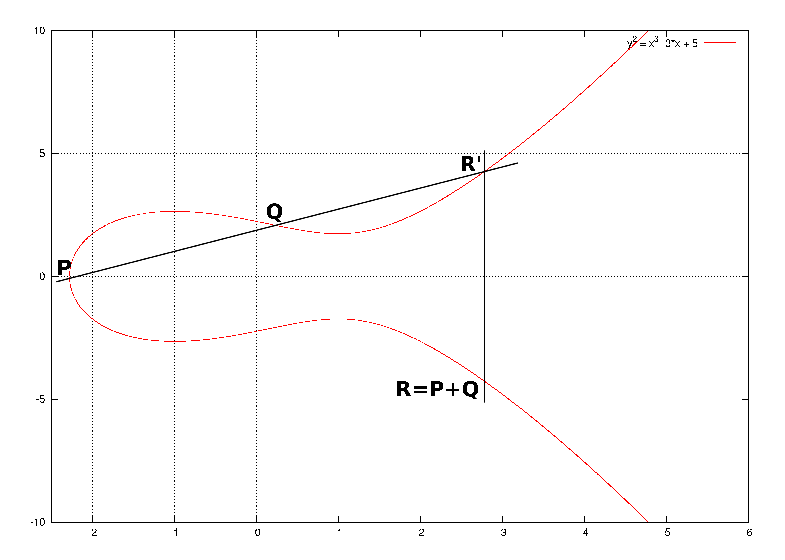
\includegraphics[width=\linewidth]{figures/ecAdd.eps}
              \caption{Adding two points}
              \label{fig:ecAdd}
          \end{figure}
      \end{minipage}
     % \hspace{0.05\linewidth}
      \begin{minipage}{0.5\linewidth}
          \begin{figure}[H]
              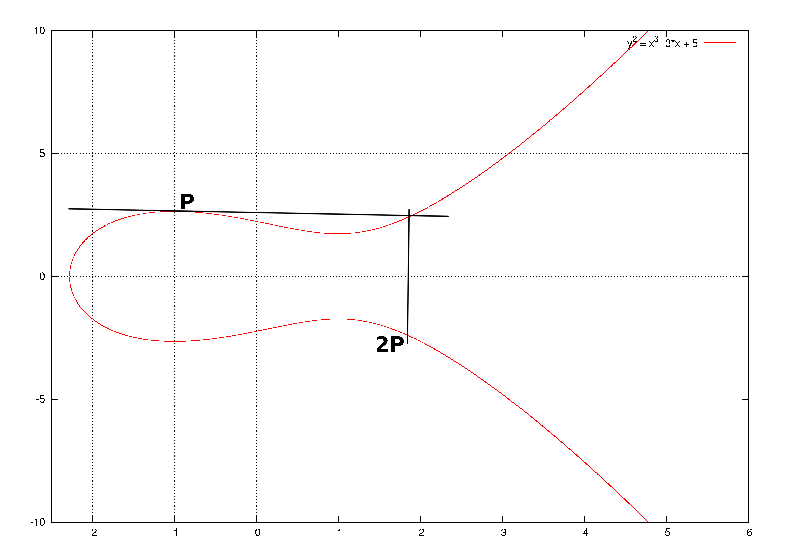
\includegraphics[width=\linewidth]{figures/doubleEC.eps}
              \caption{Doubling a point}
              \label{fig:ecDouble}
          \end{figure}
      \end{minipage}
  \end{minipage}

By defining an \gls{ec} over $\mathbb{Z}_p$, with $a, b \in \mathbb{Z}_p$, a cyclic group can be generated. The addition operation that "adds" two points on
this curve is defined by a "chord-and-tangent" rule. Figure \ref{fig:ecAdd}
shows addition of two points, while \ref{fig:ecDouble} shows adding a point to itself. It is important to note that this representation is shown in the domain
$\mathbb{R}$ for visualization - in real \gls{ec} cryptography, only elements $\pmod p$ (i.e. from the set $\mathbb{Z}_p$)
are allowed. 

FIXME: praktische gruende warum nur finite fields statt real domain: rounding errors, only finite number of points

Addition is defined as connecting points $A$ and 
$Q$, finding the intersection of the line with the \gls{ec} ($R'$) and reflecting that point across the x-axis to obtain the result $R$.
Point-doubling of $P$ is achieved in a similar way by determining the tangent of $P$, finding the intersection and reflection. Formulae to calculate x- and y-coordinates for the resulting points
for point addition $R=P+Q$ and point doubling $R=P+P$ are shown in equations \ref{adding} and \ref{doubling} respectively:

\begin{align}\label{adding}
 x_3 = (\frac{y_2-y_1}{x_2-x_1})^2-x_1-x_2, y_3=\frac{y_2-y_1}{x_2-x_1}(x_1-x_3)-y_1
\end{align}

\begin{align}\label{doubling}
 x_3 = (\frac{3x_1^2 +a}{2y_1})^2 - 2x_1, y_3=\frac{3x_1^2+a}{2y_1}(x_1-x_3)-y_1
\end{align}
Multiplication is defined as successive addition of a point to it self in the way

\begin{center}
 $kP = \underbrace{P+P+...+P}_{k-times}$
\end{center}
An imaginary point "in infinity", denoted $\infty$, serves as additive neutral element, and also belongs to the \gls{ec} by definition:

\begin{center}
 $P + \infty = \infty + P = P$
\end{center}
Negatives can be calculated easily due to the symmetric nature of the curves by swapping the sign of the y-coordinate of the point. For point $P$ with coordinates $(x, y)$, $-P$ is defined as
$(x,-y)$, thus satisfying $P + (-P) = \infty$.

\subsubsection{\gls{ecdlp}}\label{ecdp}

Based on this group operations, the \gls{ecdlp} \cite{ecdlp} can be defined as following: given an \gls{ec} $E$ over the finite field $\mathcal{F}_p$ and 2 points $P,Q$ on this curve, %FIXME: "P of order n...???"
find the integer $k$ s.t. $Q = kP$. $k$ is called the discrete logarithm of $Q$ to the base $P$.
\\
\\
To build a public key system, two users $A$ and $B$ initially agree on a set of public \textit{domain parameters}. The most important parameters are \cite{ecDP}

\begin{itemize}
 \item the order of the field, $q$
 \item the coefficients $a, b \in \mathcal{F}_p$, defining the \gls{ec}
 \item the coordinates $(x_p, y_p \in \mathcal{F}_p)$ of the \textit{base point} $P$, 
 \item the order of $P$, denoted $n$
\end{itemize}
After agreeing on this set, $A$ selects a randomly chosen integer $k_A$, calculates $P_A = k_A*P$ and sends
this point to $B$, who in turn randomly chooses $k_B$ and sends $P_B = k_B*P$ to $A$. Subsequently, booth can calculate the point $k_A*k_B*P$, which can be used
to derive a key.

\subsection{Key establishment with more communication partners}
\gls{dh} and therefor also the \gls{ecdlp} can be generalized to $n$ parties, obtaining one key in common. The key negotiation procedure for 3 parties, using
classical \gls{dh}, is
shown in figures \ref{fig:dh1} and \ref{fig:dh2}, where it is assumed that all 3 parties $A$, $B$ and $C$ already agreed upon $(p,g)$.

\begin{figure}
    \centering
    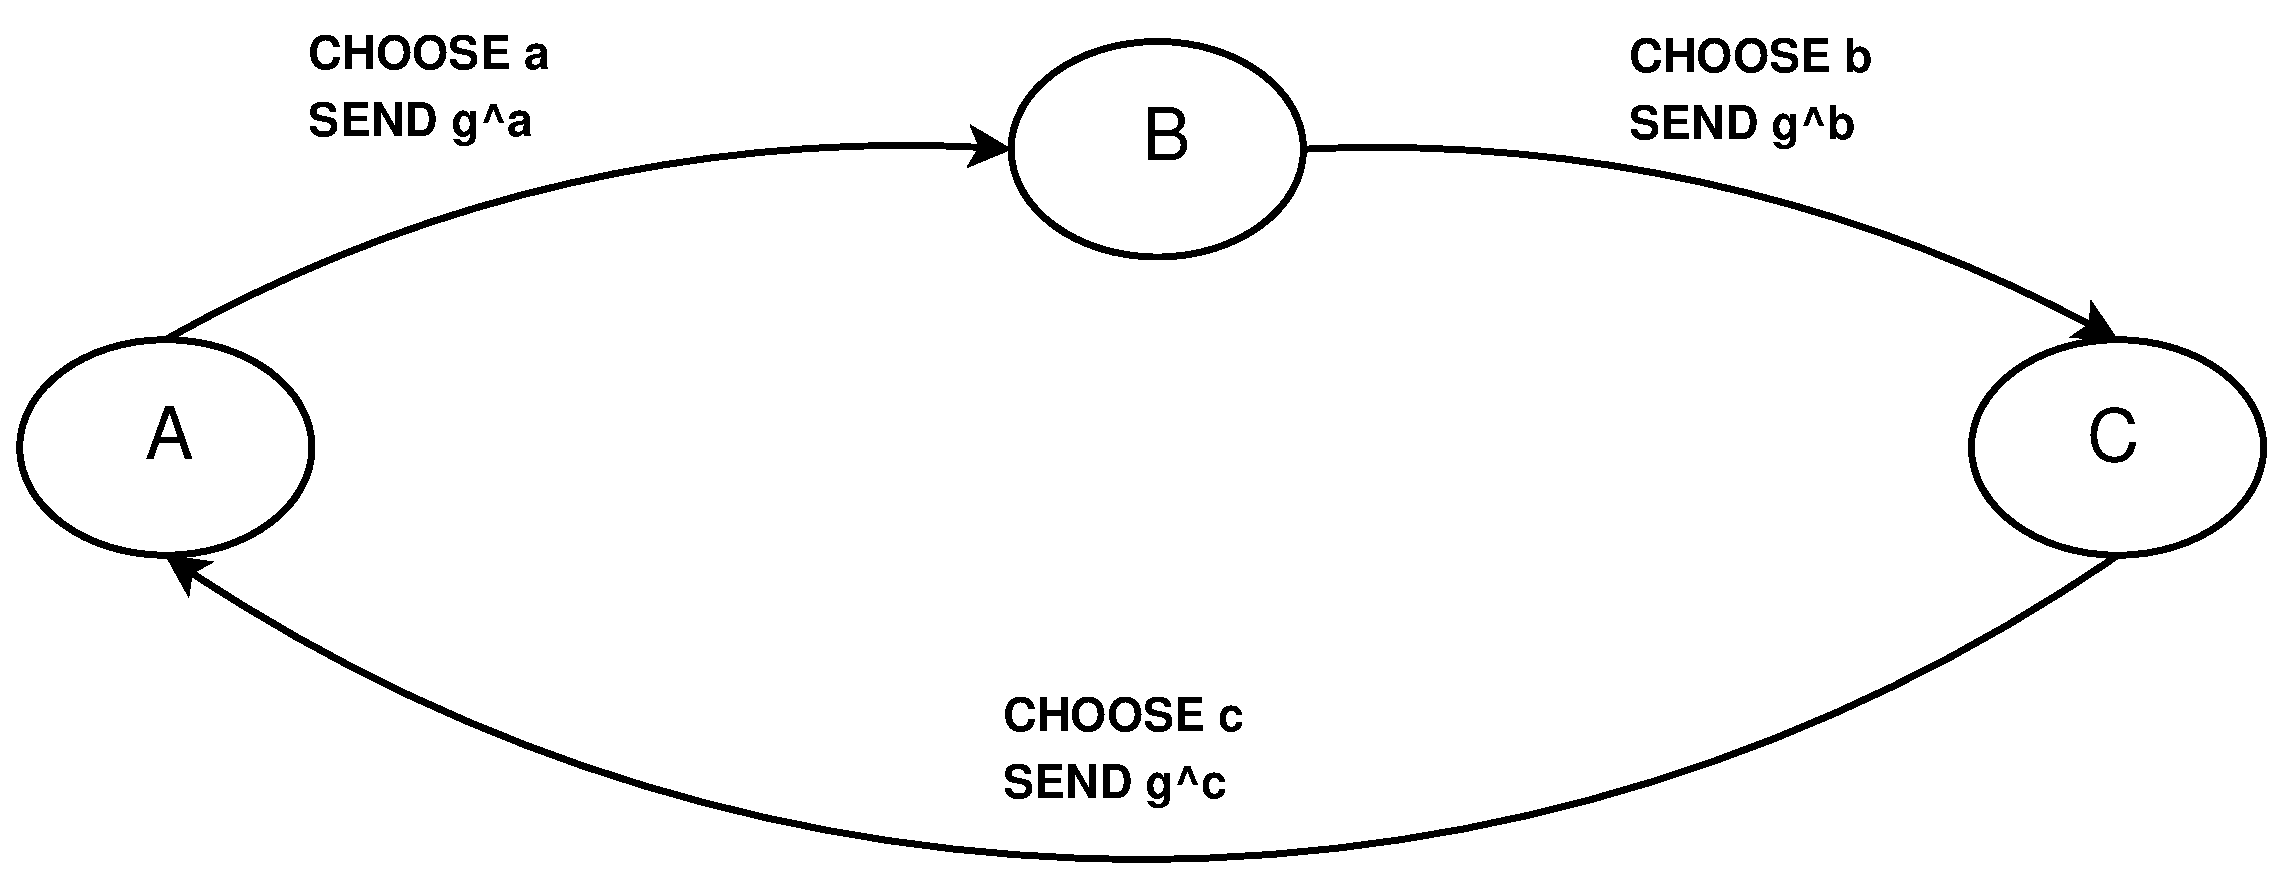
\includegraphics[width=0.8\textwidth]{figures/dh-group_round1.eps}
    \caption{DH Round 1}
    \label{fig:dh1}
\end{figure}

\begin{figure}
    \centering
    \includegraphics[width=0.8\textwidth]{figures/dh-group_round2.eps}
    \caption{DH Round 2}
    \label{fig:dh2}
\end{figure}
After finishing the second communication round, every party raises the last received value to it's own private key and thus derives the shared secret.

\begin{align}
 ((g^b)^c)^a = ((g^c)^a)^b = ((g^a)^b)^c = g^{a*b*c}
\end{align}
This algorithm can be generalized to $n$ parties, using $(n-1)$ communication rounds. Obviously, this algorithm may not be practicable for a large $n$. Additionally,
a complete new run must be executed whenever a new node joins.
\\
Additionally, this key agreement mechanism (as well as all others presented so far) uses not authentication and is therefor vulnerable to active attacks.

\subsection{RSA}

RSA, published in 1977 by Ron Rivest, Adi Shamir, and Leonard Adleman \cite{RSA} and formalized in \cite{pkcs1},
relies on the hardness of finding the prime factors of a big composite number.
In contrast to \gls{dh}, RSA is no to key agreement algorithm but can instead be used to encrypt \textit{and} sign messages. 
\\
For key generation, 
two large primes $p, q$, which should be of about same size, are chosen randomly, with $N = pq$. Additionally, a public exponent $e$ and a private exponent
$d$ are chosen s.t. they are multiplicative inverses to each other in $\pmod{\varphi(N)}$:
\begin{align}\label{ed}
 e * d \equiv 1 \pmod {\varphi(N)}
\end{align}
$\varphi(N)$, Euler's totient function, counts the number of integers in the interval $[1, N]$ which are relatively prime to $N$.
For a prime $p$, $\varphi(p) = (p-1)$, therefore for the product
$p*q$ of two different primes, $\varphi(p*q) = (p-1) * (q-1)$.
Additionally, Euler's theorem is used:
\begin{align}\label{euler}
a^{\varphi(N)} \equiv 1 \pmod N
\end{align}
The public key consists of the pair
\begin{center}
 $(N, e)$
\end{center}
and the private key of the pair
\begin{center}
 $(N, d)$
\end{center}

In practice, for the public exponent $e$ the numbers 3, 5, 17, 257 or 65537 are suggested \cite{891000}, a suitable $d$ satisfying \ref{ed} can then be found
by using the extended Euclidean algorithm.

\subsubsection{Encrypting of messages}

To encrypt, the message $M$ must be converted to an integer. Then, the sender uses the recipients public key and raises $M$ to the power of $e \pmod N$:
\begin{center}
 $C \equiv M^e \pmod N$
\end{center}
To decrypt, the receiver uses his own private key to raise $C$ to the power of $d \pmod N$:
\begin{align}\label{decrypt}
 M' \equiv C^d \equiv M^{d*e} \bmod N
\end{align}
From the way $e$ and $d$ have been chosen in \ref{ed} it follows that 
\begin{align}\label{ed2}
 e*d = k * \varphi(N) + 1, k \in \mathbb{Z} 
\end{align}
Inserting \ref{ed2} in equation \ref{decrypt} yields:
\begin{align}\label{cong}
  M' \equiv M^{k * \varphi(N) + 1} \equiv M* M^{k * \varphi(N)} \pmod N
\end{align}
By using Euler's theorem \ref{euler}, expression \ref{cong} shows that $M=M'$, i.e. decryption yields the correct value because
\begin{align*}
 M' \equiv M* M^{k * \varphi(N)} \equiv M* (M^{ \varphi(N)})^k \equiv M * 1^k \equiv M \pmod N
\end{align*} 

\subsection{Digital Signatures}\label{digitalSignatures}

Digital signatures are, as its symmetric-key \glspl{mac2} counterparts, used to provide integrity. Most digital signature schemes are based on
cryptographically secure hash functions, so the same requirements as listed in \ref{Integrity} must also hold here.
\\
\\
Nevertheless, due to the use of asymmetric keys, an important semantic difference between \glspl{mac2} and digital signatures emerges: for a \gls{mac2} 
a key is shared by at least 2 entities. A digital signature, in contrast, is generated by utilizing the private key of an entity. Therefor,
digital signatures can also provide non-repudiation.
This property allows to convince an unbiased "judge" that a message, signed by the sender, was indeed sent by this sender, i.e. the message was not
forged by a third party. This is an important difference to \glspl{mac2}, where such a behavior is not possible.

\subsubsection{RSA}

By 'reversing' the encryption process, the RSA algorithm can also be used to generate signatures of a message.
This is typically achieved by generating a hash value of the message and \textit{encrypting} that hash with the \textit{private} key. The signature is then attached to the
message. Afterwards, every entity can verify the integrity by \textit{decrypting} the signature with the \textit{public} key of the sender, calculating of
the hash of the message and comparing it to the decrypted hash.

\subsubsection{\gls{ecdsa}}

FIXME Based on the idea of Scott Vanstone, this signature algorithm is the \gls{ecc} variant of the \gls{dsa}, standardized by \gls{nist} \cite{nistECDSA}.
Analog to the \gls{ecdlp}, as shown in section \ref{ecdp}, the domain parameters are public knowledge. The signer of the message chooses a random integer $k$ and
computes the coordinates $(x_Q, y_Q)$ of a new point $Q$ by multiplying $k*P = Q$. Afterwards, $x_Q$ is converted to an integer, obtaining $r = x_Q' \pmod n$. Finally,
by using his private key $d$, $s$ is calculated:

\begin{align}\label{ecdsLabel}
s \equiv k^{-1}(h(m)+dr) \pmod n
\end{align}
This results in the tuple $(r,s)$, i.e. the signature of $m$.
\\
\\
The receiver of the message can use the domain parameters and signature to verify the integrity by calculating:

\begin{align*}
 x' \equiv s^{-1}(h(m)P + rQ) \pmod n\\
 x' \equiv s^{-1}(h(m)P + rkP) \pmod n\\
 x' \equiv P \underbrace{(s^{-1}(h(m) + rk))}_{k'} \pmod n
\end{align*}
$x'$ is converted to an integer an reduced $\pmod$ to obtain $r'$. If $r = r'$, the signature is accepted, proofing the authenticity of the message.

\subsubsection{Decryption and Authenticity Check}

\subsubsection{Attacks on CCM}

FIXME: meet in the middle attack, siehe rfc 3610

\subsection{Key lenghts}

\cite{Lenstra04keylength}

TODO: BIRTHDAY PARADOXON

\section{Attacks on Ciphers}

ciphertext-only

known-plaintext

chosen plaintext

chosen ciphertext

\subsection{Passive Attacks}

timing attacks - constant time computation

\subsection{Active Attacks}

% Such a cipher as defined above provides confidentiality, i.e. it ensures that only authorized parties are able to decrypt the message. This leads to other
% problems, namely how to determine who is authorized, i.e. how to provide authenticity, and how to assure that the message was not altered when, i.e. how to 
% provide integrity. It turns out that such a cipher is suitable for these purposes
% 
% A system is an entity that interacts with other entities, which constitute the environment for the system and
% can be other systems, humans or the physical world \cite{1335465}. Fundamental properties of communication systems
% are \textit{functionality, performance, security and dependability}. The system provides services to the user(s) 
% of the system through it's service interface, described by the functional specification. Whenever the provided service
% deviates from correct service a system failure occurs. 
% An informal definition of a dependable system is a system which delivers a service that can be justifiable trusted. More formally,
% dependability consists of the following attributes:
% \textit{Availability}, which means that the system is ready for correct service, \textit{reliability}, the continuity of correct service,
% \textit{safety}, i.e. the avoidance of catastrophic consequences \textit{integrity}, s.t. the system cannot be modified in an unwanted manner
% and \textit{maintainability}, so that the system can be repaired in the case of a failure.
% 
% In case of a secure system, another important property is \textit{confidentiality}, which means that no information is disclosed to unauthorized 
% entities.
% To achieve 
